
\documentclass[]{report}
%
\setcounter{secnumdepth}{5}

\usepackage{listings}
\usepackage{color}
\usepackage{xspace}
\usepackage{graphics}
\usepackage{graphicx,subfigure}
\usepackage[utf8]{inputenc}
\usepackage{ifthen}
\usepackage{algorithm}
\usepackage{algorithmic}
\usepackage{a4wide,amssymb,amsbsy,amsmath}
\usepackage[many]{tcolorbox}
\usepackage{tikz}
	\usetikzlibrary{calc}
	\usetikzlibrary{shapes,shadows,arrows,positioning}
	\usetikzlibrary{decorations.pathreplacing,decorations.pathmorphing}
\lstset{escapeinside={<@}{@>}}
\tolerance=1000
%% The lineno packages adds line numbers. Start line numbering with
%% \begin{linenumbers}, end it with \end{linenumbers}. Or switch it on
%% for the whole article with \linenumbers after \end{frontmatter}.
\begin{document}

%% \usepackage{lineno}


\renewcommand{\thesection}{\Roman{section}}
\renewcommand{\thesubsection}{{\color{gray}\thesection~}\alph{subsection})}
\renewcommand{\thesubsubsection}{{\color{gray}\thesubsection~}\roman{subsubsection}}
\renewcommand{\theparagraph}{{\color{gray}\thesubsubsection~}\arabic{paragraph}}

\newcommand{\comments}[1]{{\scriptsize\color{gray} #1}} % pour les commentaires

\DeclareRobustCommand{\matlab}{\texttt{MatLab}\xspace}
\DeclareRobustCommand{\mcode}[1]{\texttt{#1}\xspace}


%%%%%%%%%%%%%%%%%%%%%%%
% classique tools
\newcommand{\gras}[1]{\boldsymbol{#1}}
\newcommand{\mypar}[1]{\left(#1\right)}
\newcommand{\mya}[1]{\left\{#1\right\}}
\newcommand{\norme}[1]{\left\Vert #1\right\Vert_2}
\newcommand{\monabs}[1]{\left| #1\right|}


%%%%%%%%%% notations communes
\newcommand{\Ephaz}{\mathcal{D}}%espace des phases
\newcommand{\Eobs}{\Omega}%espace des observables

\newcommand{\Np}{n_p} % dim espace des phases
\newcommand{\Nobs}{n_r} % dim espace des observables
\newcommand{\Ns}{n_s} % dim sensors
\newcommand{\Nsnap}{N} % nombre de snapshots

%\newcommand{\flot}{\phi} % flot dynamique
\newcommand{\fdyn}{\mathfrak{f}} % fonction dynamique

%\newcommand{\velo}{\gras{u}} % champ de vitesse
\newcommand{\obs}{\gras{u}} % observable
\newcommand{\statei}{x} % comp de l'espace des phases
\newcommand{\state}{\gras{\statei}} % state de l'espace des phases
\newcommand{\freq}{\nu}
%%%%%%%%%% DMD notations
\newcommand{\Opev}{A} % Opérateur linéaire d'évolution

\newcommand{\Om}{\mathcal{K}} % matrice de Kalman
% observabilité notations
\newcommand{\dmdo}{\sigma} % DMD observability
\newcommand{\Pd}{\mathcal{S}} % Vecteur DMD observabilité = pertinence 
\newcommand{\chronos}{\xi}

% Define block styles
\newcommand{\todo}[1]{{ \center \LARGE\color{red}  [[TODO #1 ]] \\ }}    
\newcommand{\todoimage}[1]{\todo{ ** image #1 **}} 
    
\newtcolorbox[auto counter]{mytipbox}{
freelance,
colback=white,
frame code={},
interior titled code={
  \fill[rounded corners=8pt,blue!50]
    (title.south west) --
    (title.south) -- 
    ([yshift=20pt]title.south) --
    ([yshift=20pt,xshift=4cm]title.south) --
    ([xshift=4cm]title.south) --
    (title.south east) {[sharp corners] --
    ([yshift=-6pt]title.south east) -- 
    ([yshift=-6pt]title.south west) } -- cycle;
  \draw[rounded corners=8pt,gray,line width=1pt]
    (title.west|-frame.south west) --
    (title.south west) --
    (title.south) -- 
    ([yshift=20pt]title.south) --
    ([yshift=20pt,xshift=4cm]title.south) --
    ([xshift=4cm]title.south) --
    (title.south east) --
    (title.east|-frame.south east) --
    cycle;
  \node at ([xshift=2cm,yshift=4pt,anchor=south]title.south) 
    {\sffamily\Large ProTip~\thetcbcounter};  
  },
title={\mbox{}},
top=12pt,
fontupper=\sffamily\Large,
oversize=0.5cm,
before={\vskip24pt\par\noindent},
after={\par\vskip12pt}
}


\newcommand{\tipbox}[1]{  { \begin{mytipbox} #1 \end{mytipbox} }  }   

\newtcolorbox[auto counter]{mydefbox}{
freelance,
colback=white,
frame code={},
interior titled code={
  \fill[rounded corners=8pt,green!30]
    (title.south west) --
    (title.south) -- 
    ([yshift=20pt]title.south) --
    ([yshift=20pt,xshift=4cm]title.south) --
    ([xshift=4cm]title.south) --
    (title.south east) {[sharp corners] --
    ([yshift=-6pt]title.south east) -- 
    ([yshift=-6pt]title.south west) } -- cycle;
  \draw[rounded corners=8pt,gray,line width=1pt]
    (title.west|-frame.south west) --
    (title.south west) --
    (title.south) -- 
    ([yshift=20pt]title.south) --
    ([yshift=20pt,xshift=4cm]title.south) --
    ([xshift=4cm]title.south) --
    (title.south east) --
    (title.east|-frame.south east) --
    cycle;
  \node at ([xshift=2cm,yshift=4pt,anchor=south]title.south) 
    {\sffamily\Large Definition~\thetcbcounter};  
  },
title={\mbox{}},
top=12pt,
fontupper=\sffamily\Large,
oversize=0.5cm,
before={\vskip24pt\par\noindent},
after={\par\vskip12pt}
}


\newcommand{\defbox}[2]{  { \begin{mydefbox} {\color{green}#1:} #2 \end{mydefbox} }  }   


\definecolor{mygreen}{RGB}{28,172,0} % color values Red, Green, Blue
\definecolor{mylilas}{RGB}{170,55,241}
\lstset{language=Matlab,%
    %basicstyle=\color{red},
    breaklines=true,%
    morekeywords={matlab2tikz},
    keywordstyle=\color{blue},%
    morekeywords=[2]{1}, keywordstyle=[2]{\color{black}},
    identifierstyle=\color{black},%
    stringstyle=\color{mylilas},
    commentstyle=\color{mygreen},%
    showstringspaces=false,%without this there will be a symbol in the places where there is a space
    numbers=left,%
    numberstyle={\tiny \color{black}},% size of the numbers
    numbersep=9pt, % this defines how far the numbers are from the text
    emph=[1]{end},emphstyle=[1]\color{black}, %some words to emphasise
    %emph=[2]{word1,word2}, emphstyle=[2]{style},    
}



	
\title{Introduction to \matlab.}


\author{Florimond Gu{\'e}niat}

%\authorrunning{Short form of author list} % if too long for running head



\maketitle





\chapter{Quick tour \matlab}
	The objective of these tutorial are to illustrate the ENG 4XXX courses as well at to help you to learn quickly how to numerically solve problems.
	
	It will hence provide to the reader the first concepts, not only behind \matlab, but as well on how to code and how to solve problems.
	
	The emphasis here is “learning by doing”. Therefore, the reader should not to read these documents without a computer close-by.

%%%%%%%%%%%%%%%%%%%%%%%%%%%%%%%%%%%%%%%%%%%%%%%%
%%%%%%%%%%%%%%%%% SECTION %%%%%%%%%%%%%%%%%%%%%%
%%%%%%%%%%%%%%%%%%%%%%%%%%%%%%%%%%%%%%%%%%%%%%%%
\section*{Legal stuff}
\matlab is a registered trademark of MathWorks, Inc. 




%%%%%%%%%%%%%%%%%%%%%%%%%%%%%%%%%%%%%%%%%%%%%%%%
%%%%%%%%%%%%%%%%% SECTION %%%%%%%%%%%%%%%%%%%%%%
%%%%%%%%%%%%%%%%%%%%%%%%%%%%%%%%%%%%%%%%%%%%%%%%
\section{About \matlab}
	%%
	% subsection
	%%
	\subsection{What is the use of \matlab ?}
		\matlab~(for MATrix LABoratory) aims at delivering quickly some results on a user-defined problem.

		It shines, as expected from the name, when it involves linear algebra, i.e., operations on matrices.
		\matlab makes the manipulaiton of matrices really easy, as it will hopefully been demonstrated through these notes.

		\matlab has several main advantages compared to language like C/C++ or Fortran are:
		\begin{itemize}
			\item No compilation \\
				\comments{a script can be executed directly.}
			\item The prompt \\
				\comments{results can be analyzed right away.}				
			\item Simplicity \\
				\comments{the learning curve is low}
			\item Portability
				\comments{a script will work on any \matlab, and on any platform: Linux, Mac or Windows.}
			\item Built-in functions
				\begin{itemize}
					\item Integration \\
						\comments{solving equations is \emph{relatively} easy}
					\item Visualization\\
						\comments{plotting the results in one command}
					\item Tool-box\\
						\comments{many tools dedicated to problems already exist}
					\item Data-Analysis \\
						\comments{basic and advanced tools for data-analysis and machine learning are already implemented}
				\end{itemize}
		\end{itemize}

		The negative points are mostly:
		\begin{itemize}
			\item Sub performance \\
				\comments{No compilation means less efficiency}
			\item Not open source \\
				\comments{The results can not easily be checked}
			\item {\color{red} Price}
				\comments{It can be up to $1800\pounds$}
		\end{itemize}

	%%
	% subsection
	%%
	\subsection{Equivalent of \matlab }

		Octave and SciLab are almost identical to \matlab. A \matlab script would work on these two others open-source and free softwares.

		Most of the tips can also be applied to python, especially when the packages scipy and numpy (for scientific and engineering computations) are used.


%%%%%%%%%%%%%%%%%%%%%%%%%%%%%%%%%%%%%%%%%%%%%%%%
%%%%%%%%%%%%%%%%% SECTION %%%%%%%%%%%%%%%%%%%%%%
%%%%%%%%%%%%%%%%%%%%%%%%%%%%%%%%%%%%%%%%%%%%%%%%
\section{Hello, World!}
	Let's print in the console the "Hello, World!".
	\tipbox{
		When starting to learn a programming language, trying to make a program that print "hello, World!" is usually a good idea.
		
		It will show the basics of: 
		\begin{itemize}
			\item installing the language/program
			\item the syntax of the language
			\item running the language/program
		\end{itemize}
	}
	%%
	% subsection
	%%
	\subsection{Starting with \matlab}
		\subsubsection{Launch \matlab}
		Click on the icon, duh! Fig.~\ref{fig-matlab_icon} represents the icon.
		\begin{figure}[h!]
			\center
			
\includegraphics[width=0.45\linewidth]{./fig/icon_matlab.PNG}
			\caption{
				The \matlab icon (in super big).
			}
			\label{fig-matlab_icon}
		\end{figure}

		\subsubsection{Organization of the typical \matlab window}
		When clicking on the icon, \matlab will start. 
		The main window opens, see Fig.~\ref{fig-matlab}. It is separated in a few important sections:
		\begin{itemize}
			\item the command windows \\
				\comments{This is the command prompt}
			\item current folder \\
				\comments{It lists the files}
			\item the Workspace \\
				\comments{It gives details on the objects present in memory}
			\item the editor \\
				\comments{this is where you can write a script}
			\item the ribbon \\
				\comments{It gives access to properties, functions, editor, etc. Similar in spirit to Words and Excel.}
		\end{itemize}

		\begin{figure}[h!]
			\center
			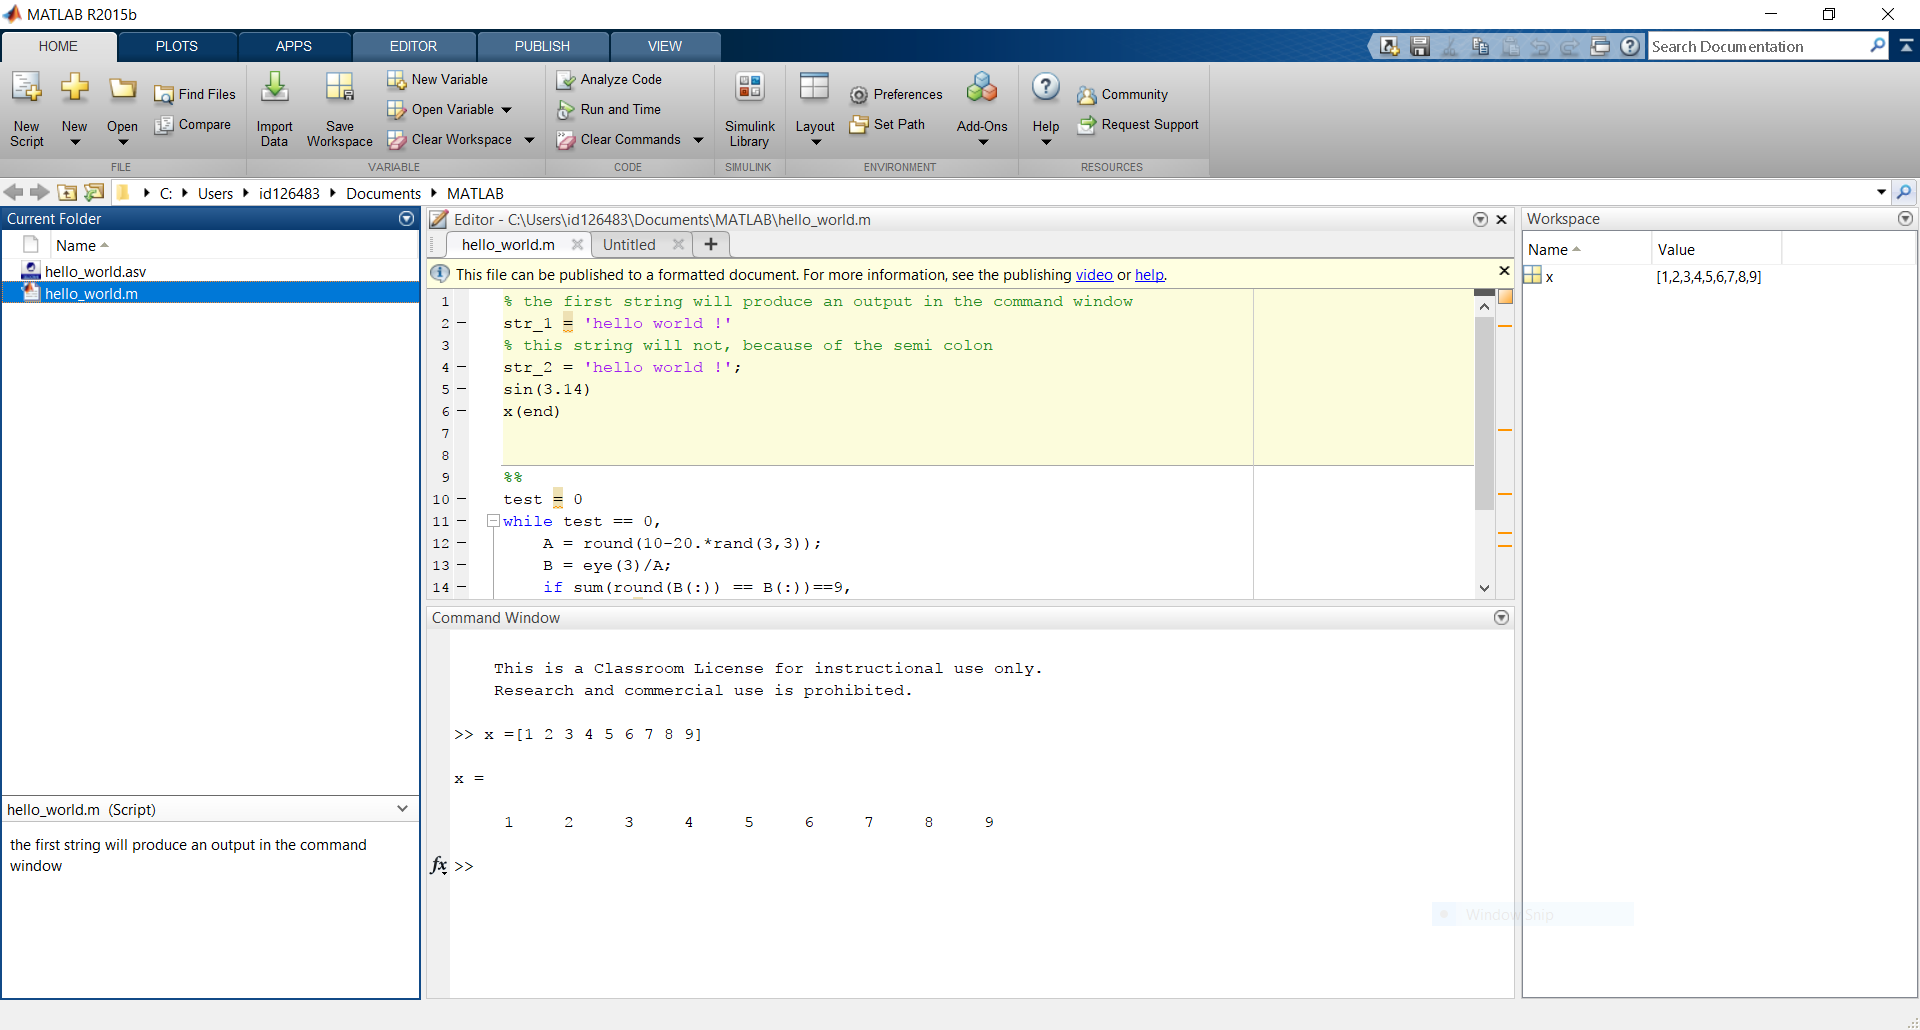
\includegraphics[width=0.95\linewidth]{./fig/matlab.PNG}
			\caption{
				\matlab just after being opened.
			}
			\label{fig-matlab}
		\end{figure}
	%%
	% subsection
	%%
	\subsection{How to print "hello world"}

		Click on the Command Window, and type "hello world".
		You will see:
		\begin{figure}[h!]
			\center
			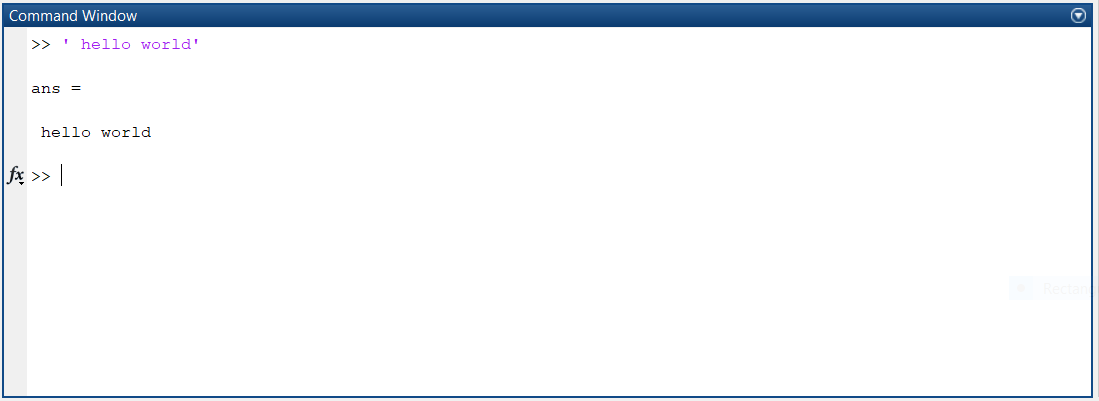
\includegraphics[width=0.85\linewidth]{./fig/hello_world.PNG}
			\caption{
				How to print 'hello world'.
			}
			\label{fig-hellow_world}
		\end{figure}
		

		\matlab~printed the 'Hello World', congratulations !

		One line was enough to get the desired output.
		This shows that \matlab is very efficient at getting quickly some results. 
		\medskip
		
		In the following, instead of print screen, we will show the results and the commands as:
\begin{lstlisting}
>> 'Hello World'
ans =
Hello World
\end{lstlisting}

		
		'Hello World' has been assigned to a variable named \mcode{ans}.

		\defbox{Variable}{A variable is essentially a name that is associated with a value. 

		Values can be of several types:
		\begin{itemize}
		\item results, such as string, numbers or matrices: \mcode{x = 3.}
		\item functions, for instance \mcode{sin} is a built-in function
		\item complex objects, for instance, a plot
		\end{itemize}
		They are usually assigned with the sign "="
		}

		\tipbox{\mcode{ans} is short for answer. 

			With \matlab, the results of the command is always stored in the variable \mcode{ans}, except if it is assigned to a given variable. Consequently, the command \mcode{ 1+1}  will affect the variable \mcode{ans}, but \mcode{x=1+1} will not, and \mcode{2} will be assign to \mcode{x}. 

			\mcode{ans} can be re-used in the prompt: \mcode{x = ans+1}!
		However, a good practice is to assign the result to a user-defined variable.
		}


		Trying without the quotes leads to:
\begin{lstlisting}
>> Hello World
<@{\color{red}Undefined function or variable 'Hello'.}@>
\end{lstlisting}
		plus some help.

		Hello World is understood by \matlab as a function/variable and then an option for this function.
		\matlab hence thinks that Hello is something that already exists ; it is not the case here. As a consequence, an error follows.

		The main reason behind that is that the goal here is to print a string.

		\defbox{String}{A string is a chain of characters. It is \emph{not} a number. 

		It has to be between quotes: 'some text' or double quotes: "some text". 
		For example, 'Lorem ipsum dolor sit amet' is a chain or characters.

		But it is not that easy. \mcode{s = '45'} is the chain of characters '4' and '5'. But \mcode{n = 45} is the number 45. \mcode{s} and \mcode{n} are different.  

		}

		\tipbox{How to put a quote in a string ? For instance,
			
			Having \mcode{s ='nah, can't do'} is not obvious, as \matlab will interprete the quote in "can't" as the end of the string.

			To solve the issue, double it ! \mcode{s = 'nah, can''t do} will work perfectly.
		}
		Let's try now to add a semi colon at the end of the line:
\begin{lstlisting}
>> 'Hello World';
>>
\end{lstlisting}
		Nothing is printed in the command prompt.

		\tipbox{
		Do not forget the semi-colon ";" at the end of lines !

		It is not a big deal when dealing with small matrices and small vectors.
		But when an image is being manipulated, it means that \matlab is manipulated a matrix with dimension around $1000\times1000$.
		Forgetting the ";" sign means that \matlab will show around a \emph{million} numbers every line of a script!
		}
		\defbox{Command prompt}{The command prompt is the $>>$ sign. 
		Command Prompt is a command line interpreter. It is used to execute entered commands. 
		Once enter is hit, \matlab will interpret the command, and send back any results.
		}
		One of the most important tip to remember: \matlab will always print the result of a line if it does not have a ";" at the end of the line.


%%%%%%%%%%%%%%%%%%%%%%%%%%%%%%%%%%%%%%%%%%%%%%%%
%%%%%%%%%%%%%%%%% SECTION %%%%%%%%%%%%%%%%%%%%%%
%%%%%%%%%%%%%%%%%%%%%%%%%%%%%%%%%%%%%%%%%%%%%%%%
\section{\matlab as a calculator}
	\matlab can be used as a calculator. The prompt allows to interact directly with variables, quantity, and to do computations with them.
	%%
	% subsection
	%%
	\subsection{Algebra}
		After clicking on the prompt, let's try some simple calculations:
\begin{lstlisting}
>> 4+3
ans =
7
>> 4*3
ans =
12
\end{lstlisting}
		It behaves as a calculator would.

		\matlab respects the BODMAS (Brackets, Order, Division/Multiplication, Addition/Subtraction). 

		\defbox{BODMAS}{It stands for Brackets, Order, Division/Multiplication, Addition/Subtraction.
			\begin{enumerate}
				\item start with resolving inside of the brackets: \\ $3\times (4+2) \times 4^2 + 1 = 3\times 6 \times 4^2 +1$
				\item then resolve orders (powers, roots) : \\ $ 3 \times 6\times 4^2 +1 = 3\times 6 \times 16 +1  $.
				\item then resolve division/multiplication : \\
					$3\times 6 \times 16 +1 = 288 $
				\item then finish with addition/substraction: \\
					$288+1 = 289$
			\end{enumerate}
		}
		Let's try a few different operations !
\begin{lstlisting}
>> (4+3)*2
ans =
14
>> 4+3*2
ans =
10
\end{lstlisting}

	%%
	% subsection
	%%
	\subsection{Details on variables}
		\subsubsection{\mcode{ans}}
			As seen before, \mcode{ans} can be used to store a result, but it will be overwritten every time a command is executed:
\begin{lstlisting}
>> 2+2
ans =
4
>> ans+2
ans =
6
>> ans+2
ans =
8
\end{lstlisting}

		\subsubsection{Creation and re-assignement}
			Variable can be easily created and assigned with the sign "=". 
\begin{lstlisting}
>> x = 2+2
x =
4
>> x+2
ans =
6
>> x*5
ans =
10
\end{lstlisting}

		\subsubsection{Naming convention}
			A variable name can be anything, such as \mcode{goodnameforavariable} or  \mcode{GoodNameForAVariable}, or  \mcode{good\_name\_for\_a\_variable}.
			However:
			\begin{itemize}
				\item it cannot start with \_
				\item it cannot start with a number
				\item a few names are protected
			\end{itemize}

			\tipbox{Try to use clever name for variables, it will help to understand the code.

				If all the results are named \mcode{result\_1,result\_2,result\_3}, it is hard to know what they should contain.

				On the contrary, when dealing with the variable \mcode{name\_city}, it is expected to be a string and having a proper name.

				In a similar way, the variable \mcode{motor\_freq} probably contains a number.

				Also, if the piece of code uses the variable \mcode{price\_pond}, the variable \mcode{price\_dollar} and the variable \mcode{rate\_dollar2pound}, them the line \mcode{price\_pound = rate\_dollar2pond * price\_dollar} is pretty explicit.
				If the variables where instead named \mcode{x,y,z}, then the line \mcode{x = y*z} is much more cryptic.
			}
			The choice of a name is important! 
			For instance, \mcode{x} is good for an unknown, \mcode{s} if its value is expected to be a string, \mcode{v} if it is a vector... 
			More complex names can be used, such as \mcode{x\_problem\_1}. 
			
			Try to be consistent thorough the piece of code !

			A few tips:
			\begin{itemize}
				\item Use different names for different results
				\item Use a name that is meaningfull (e.g. \mcode{str\_name} if the variable is assigned with a chain of character that is a name)
				\item Consequently, avoid unecessary use of index (e.g. \mcode{result\_1, result\_2} etc.)
			\end{itemize}
			\tipbox{
				Many naming convention exist.
				
				However, the following name convention is fine: \\
				\begin{itemize}
					\item \mcode{UpperCamelCase} for functions: \mcode{MyFunction}
					\item \mbox{\mcode{CAPITALIZED\_WITH\_UNDERSCORES}} for constants \mcode{Pi=3.14}
					\item \mbox{\mcode{lowercase\_separated\_by\_underscores}} for other variables \mcode{name\_of\_univ = 'BCU'}.
				\end{itemize}
					}

		\subsubsection{Reassignement}
			Updating a variable is handy: one might want to change the variable \mcode{year} from \mcode{2017} to \mcode{2018}.

			A variable can be easily updated, by reassigning a new value to it. It hence uses the sign "=".
			For instance:
\begin{lstlisting}
>> x = 2+2
x = 
4
>> x = x + 5
x =
9
>> x = 0
x =
0
\end{lstlisting}

	%%
	% subsection
	%%
	\subsection{Workspace}
		When a variable is created, it is available in the \emph{workspace}.
		It is the area (usually) on the right.
		It allows to:
		\begin{itemize}
			\item show what variables are currently known to \matlab
			\item know what is present in the memory
			\item indicate what there is in the variables
			\item eventually modify the content of a variable
		\end{itemize}
		\begin{figure}
			\center
			\begin{tikzpicture}
				\node at (0,0) {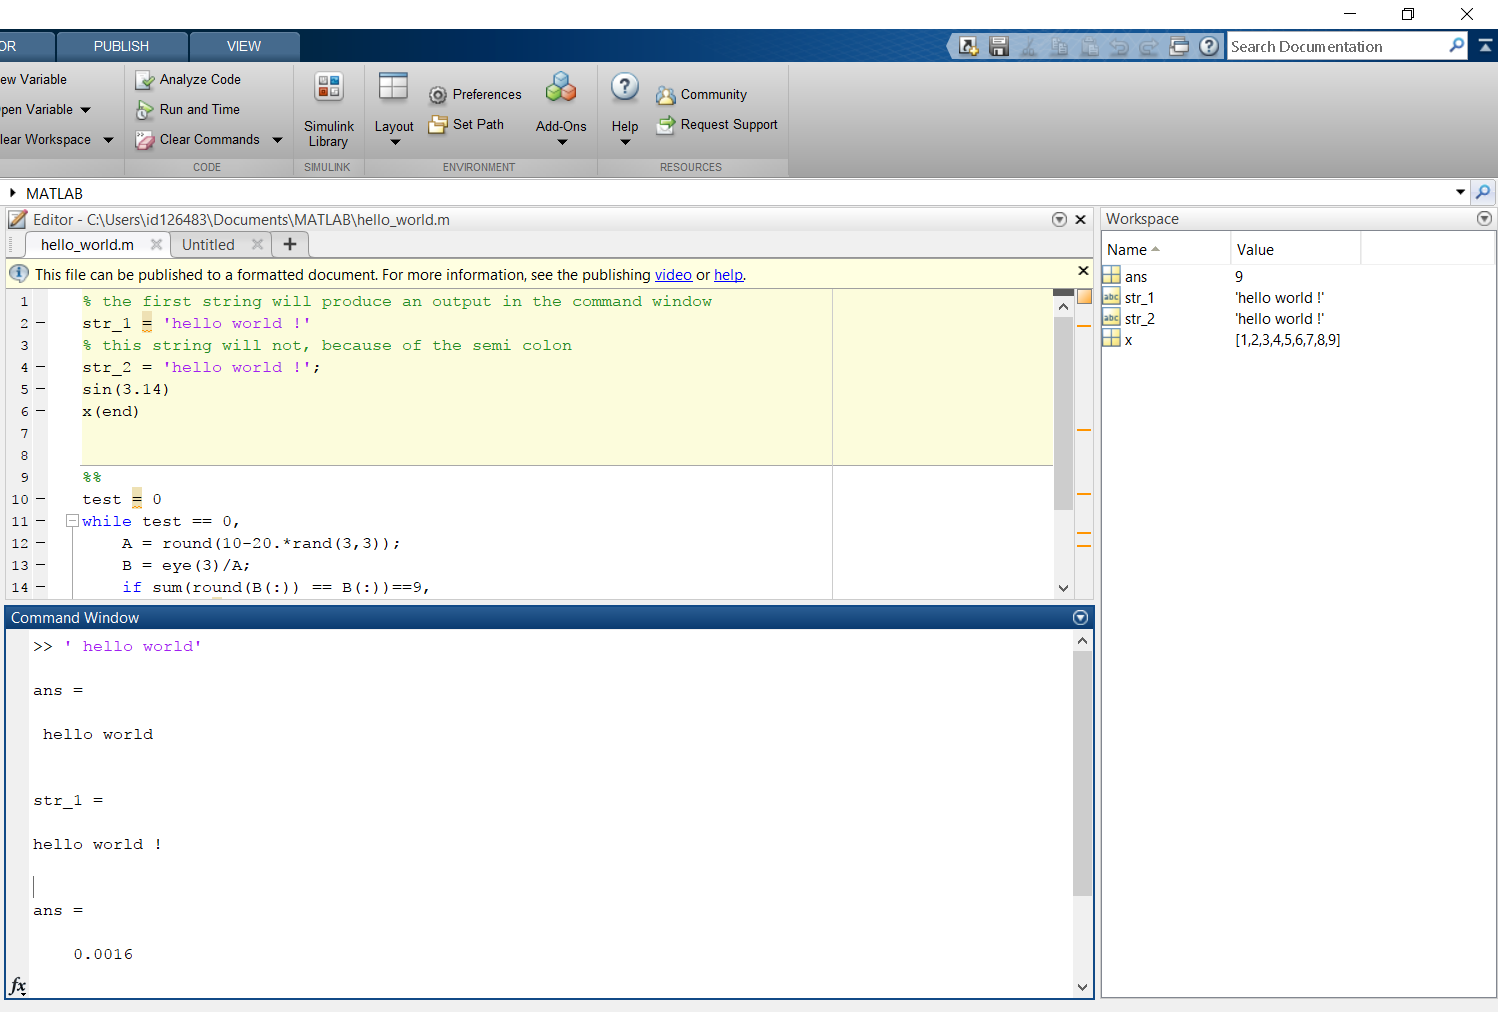
\includegraphics[width=0.95\linewidth]{./fig/workspace_zoom.PNG}};
				\draw[very thick,red,->] (2,0) -- (3.5,2.5);
			\end{tikzpicture}
			\caption{
				The workspace in \matlab. Here are the variables \mcode{ans, str\_1, str\_2} and \mcode{x} as well as their contents.
			}
			\label{fig-workspace}
		\end{figure}	
	%%
	% subsection
	%%
	\subsection{Entering multiple commands per line}
		It is possible to enter multiple commands per line. 
		Use commas "," or semicolons ";" for that ; the commas will \emph{not} suppress the outputs.

		\tipbox{Try to avoid multiple commands per line.
			
		Most of the time, it makes the code harder to read, especially if there is not a good reason to do so.

		Nevertheless, it can make sense write a few commands per line when assigning a variables that are related.
		}
\begin{lstlisting}
>> x = 2 ; y = 3 ; z = 4 ;
>> x = 2 ; y = 3 , z = 4 ;
y = 
3
>> x = 2 , y = 3 , z = 4 ,
x = 
2
y = 
3
z = 
5
\end{lstlisting}

	%%
	% subsection
	%%
	\subsection{Basic arithmetic}
		Basic arithmetic operators are pretty classic, and be found in Tab.~\ref{tab-basic_arithmetic}:
		\begin{table}[h!]\caption{Arithmetic operators}
			\label{tab-basic_arithmetic}
			\center
			\begin{tabular}{|l|c|c|}
				\hline
				operation & command & exemple \\
				\hline
				addition & + & 3+4 \\
				soustraction & - & 3-4 \\
				multiplication & * & 3*4 \\
				division & / & 3/4 \\
				power & \^{} & 2 \^{} 4 \\
				\hline
			\end{tabular}
		\end{table}

	%%
	% subsection
	%%
	\subsection{Built-in functions}
		One of the strengths of \matlab is that many functions are already available.
		One can think of common functions like sine or exponential, but \matlab also provides more complex functions like \mcode{imread}, that will import pictures, or \mcode{svd}, that will do some modal decomposition of a table of data.

		\subsubsection{How to find a function or a command ?}
			When looking for something, hit the help button.
			For instance, if one wants to look for the sine function:

		\begin{figure}
			\center
			\subfigure[]{
				\begin{tikzpicture}
					\node at (0,0) {
						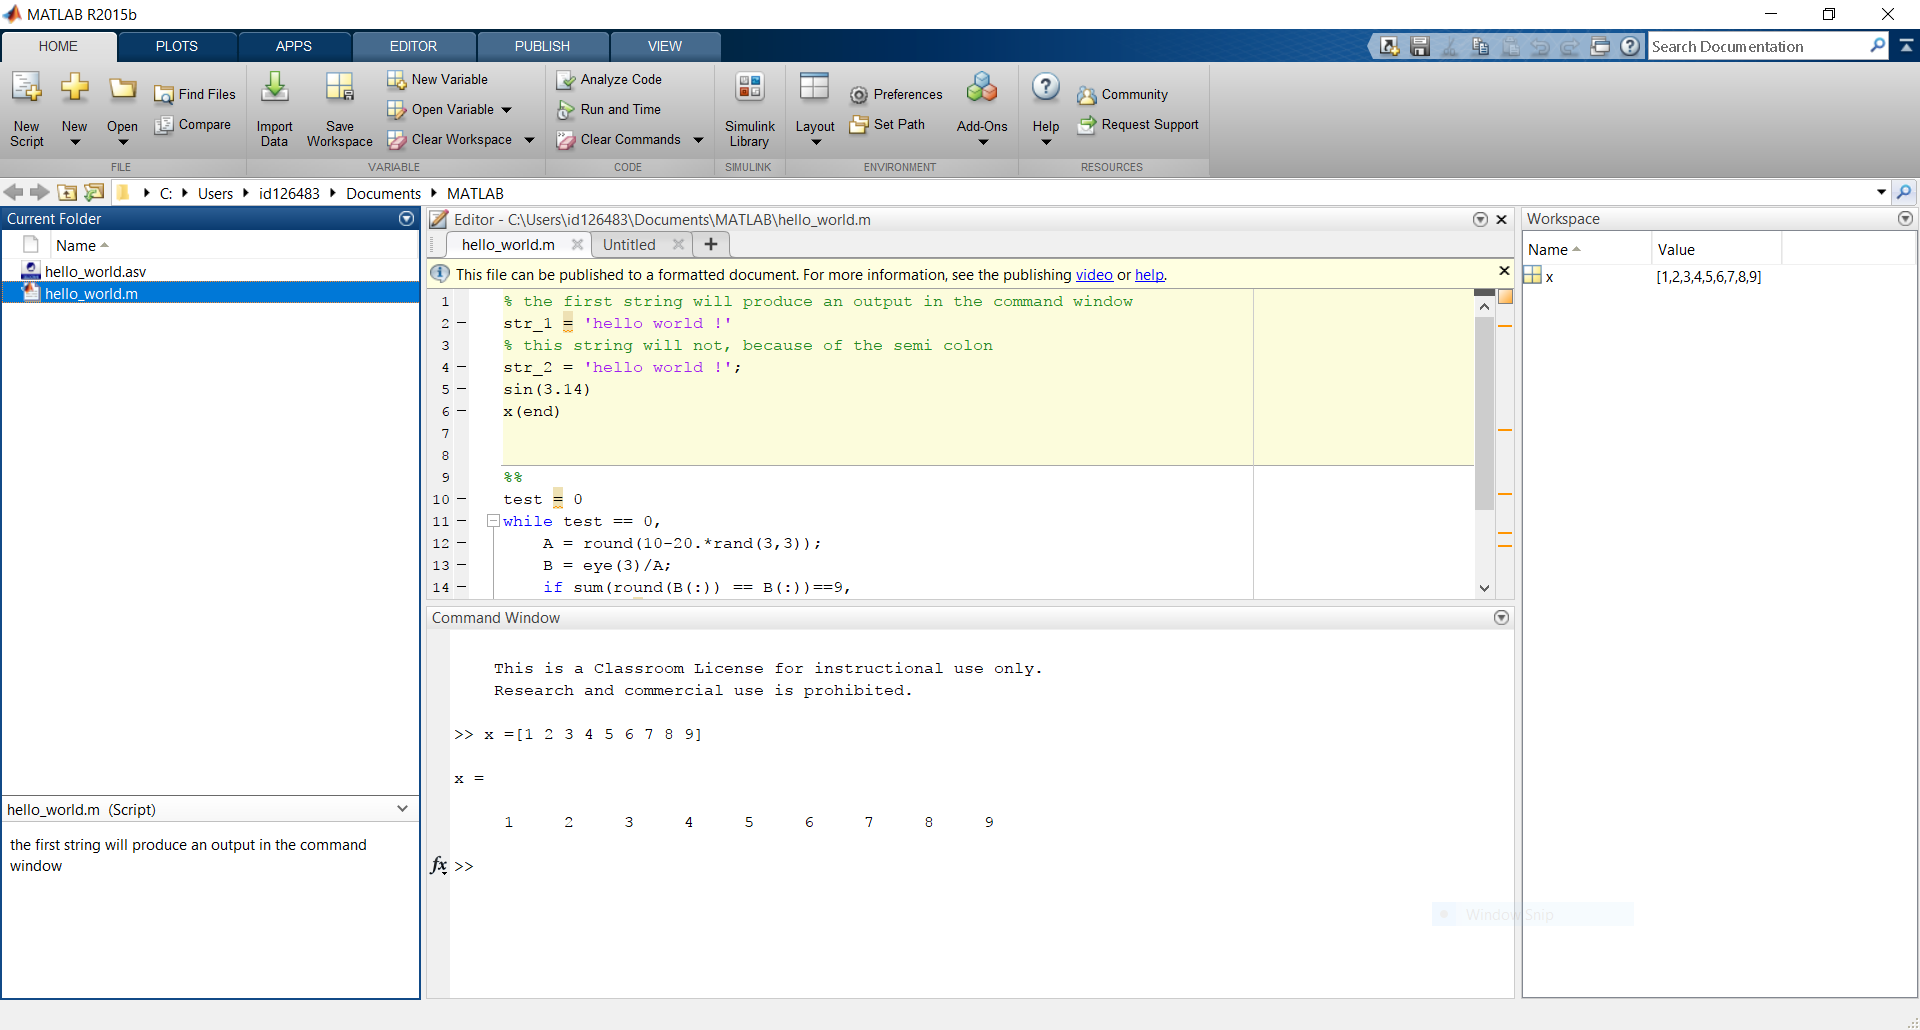
\includegraphics[width=0.95\linewidth]{./fig/help.PNG}
					};
					\draw[very thick, red, ->] (-1.45,1) -- ++(2,2) node[below, midway, rotate=45]{click here, duh};
				\end{tikzpicture}
			}

			\subfigure[]{
				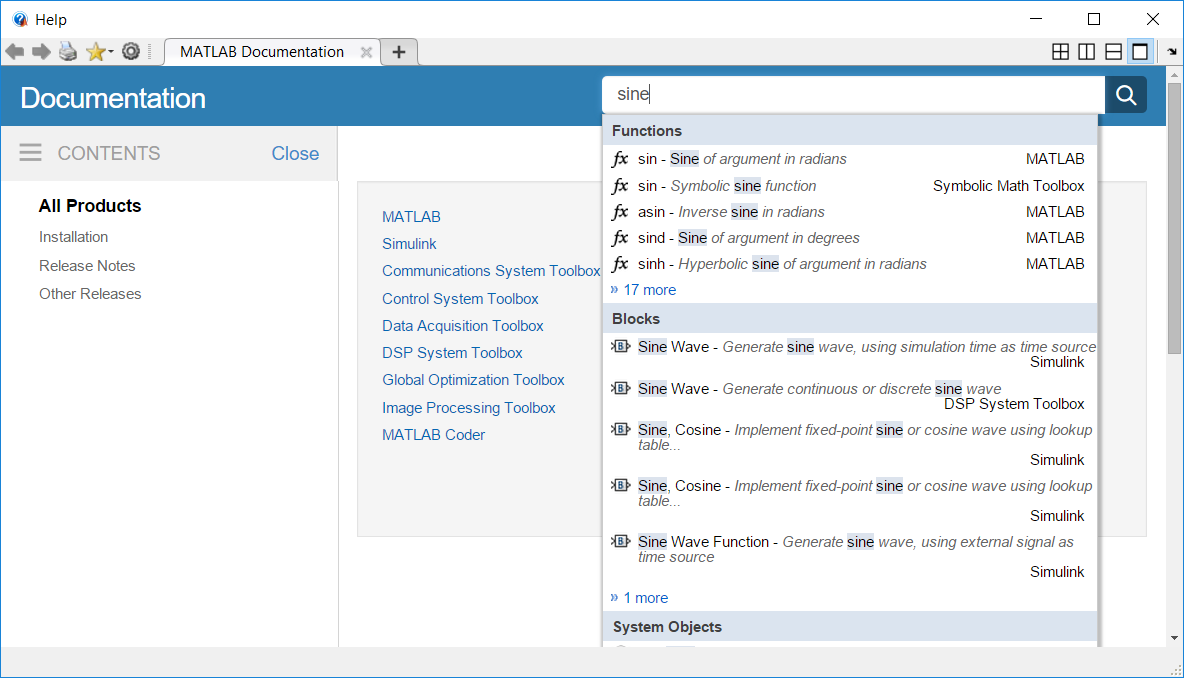
\includegraphics[width=0.95\linewidth]{./fig/sine_help.PNG}
			}
			\caption{
				Looking for sine in the help. a): where the help is. b): how to use it.
			}
			\label{fig-help}
		\end{figure}	


			\tipbox{Use the help! It is \emph{very} useful and one will mostly find any function/tool/infos that is needed.
			
			Usually, the help contains a few examples. Do not hesitate to read them carefully, and to try them.
			They will help understanding how to use the functions and properties of \matlab.
			
			There is also a "See Also" section that can be useful when looking for a particular topic.
	}
	
		\subsubsection{Using a function}
			Calling a function is relatively easy and intuitive. Let's take the sine function as an illustration. 
\begin{lstlisting}
>> sin(3.14)
ans =
0.0016
\end{lstlisting}

			\helpbox{sin}
			\matlab is asked to evaluate the function \mcode{sin} in $3.14\approx \pi$. 
			For that, the argument just has to be provided between the parenthesis.
			\tipbox{
			Trigonometric functions in \matlab are in radiant. \mcode{sin(360)} is hence different from $0$ but rather close to $0.96$.
			
			In a similar spirit, \mcode{log} in \matlab is the natural logarithm, and not the $\log$ in base 10.
			}
			Typical functions are available with somewhat explicit names, see Tab.~\ref{tab-funcs_matlab}. 
			Similarly, many useful constants for the engineer are implemented in \matlab, see Tab.~\ref{tab-consts_matlab}.
			\begin{table}[h!]
				\caption{A few function names in \matlab. Many others are already implemented in \matlab.}
				\label{tab-funcs_matlab}
				\center
				\begin{tabular}{|l|c||l|c||l|c|}
					\hline
					Trigonometry & name & Stats & name & Misc. & name\\
					\hline
					sine & sin  &
						mean & mean &
						square root & sqrt \\
				
					cosine & cos &
						maximum & max &
						absolute value & abs \\

					exponential & exp &
						minimum & min &
					round up & ceil \\		
			
					natural logarithm & log &
						standard dev. & std &
						conjugate & conj \\
		
					\hline
				\end{tabular}
			\end{table}

			\begin{table}[h!]
				\caption{A few useful constant names in \matlab.}
				\label{tab-consts_matlab}
				\center
				\begin{tabular}{|l|c|}
					\hline
					$\pi\approx 3.14$ & \mcode{pi} \\
					$i = \sqrt{-1} $ & \mcode{i} \\
					$i = \sqrt{-1} $ & \mcode{j} \\
					$\infty$ & \mcode{Inf }\\
					Not a Number & \mcode{NaN} \\
					\hline
				\end{tabular}
			\end{table}

%%%%%%%%%%%%%%%%%%%%%%%%%%%%%%%%%%%%%%%%%%%%%%%%
%%%%%%%%%%%%%%%%% SECTION %%%%%%%%%%%%%%%%%%%%%%
%%%%%%%%%%%%%%%%%%%%%%%%%%%%%%%%%%%%%%%%%%%%%%%%
\section{Let's solve a real problem}

	\paragraph*{Problem}
		\label{problem-julie}
		Julie's car's odometer reading was 35201km when she last filled the fuel tank. 
		Yesterday she checked it again and it read 35403km. Checking the tank, the car used 11 liters of gas to do so.
		If her car's gas tank holds 35 liters, how long can she drive before running out of gas? 

	\paragraph*{Solution using \matlab as a calculator}
		How much has she driven ?
\begin{lstlisting}
>> 35403 - 35201
ans =
202
\end{lstlisting}
		How much distance per liter of gas ?
\begin{lstlisting}
>> 202/11
ans =
18.3636
\end{lstlisting}
		How much gas is left in the tank ?
\begin{lstlisting}
>> 35 - 11
ans =
24
\end{lstlisting}
	Distance she can drive:
\begin{lstlisting}
>> 24 * 18.3636
ans =
440.7264
\end{lstlisting} 

	\paragraph*{Solution with variables}
	The same code can be scripted, see Chap.~\ref{chap-code}, Sec.~\ref{sec-script}. It means that we would just have to replace the value in the first three lines to update the whole code. 

\begin{lstlisting}
>> odormeter_before = 35201 ;
>> odormeter_after = 35403 ; 
>> used_gas = 11 ;
>> distance = odormeter_after - odormeter_before ;  
>> distance_per_liter = distance/used_gas ;
>> tank_capacity = 35;
>> estimated_distance = (tank_capacity - used_gas) * distance_per_liter
440.7264
\end{lstlisting}



%%%%%%%%%%%%%%%%%%%%%%%%%%%%%%%%%%%%%%%%%%%%%%%%
%%%%%%%%%%%%%%%%% SECTION %%%%%%%%%%%%%%%%%%%%%%
%%%%%%%%%%%%%%%%%%%%%%%%%%%%%%%%%%%%%%%%%%%%%%%%
\section{What to remember}
	\matlab is basically a powerful calculator.

	%%
	% subsection
	%%
	\subsection{Key example}
		Let's summarize in a few examples everything we have seen.
\begin{lstlisting}
>> year = 2018;
>> next_year = year + 1
next_year = 
2019
>> angle = pi ;
>> ( 2.*cos(angle) + 1.) ^2 
ans = 
9.0
\end{lstlisting}


%%%%%%%%%%%%%%%%%%%%%%%%%%%%%%%%%%%%%%%%%%%%%%%%
%%%%%%%%%%%%%%%%% SECTION %%%%%%%%%%%%%%%%%%%%%%
%%%%%%%%%%%%%%%%%%%%%%%%%%%%%%%%%%%%%%%%%%%%%%%%
\section{Exercices}
	%%
	% subsection
	%%
	\subsection{On Variables}
		\begin{enumerate}
			\item Create the variables \mcode{x,y,z} assigned with $1$, $2$ and $3$.
			\item Create the variable \mcode{sum\_xyz} that is the sum of \mcode{x,y} and \mcode{z}.
			\item Propose a name for a variable that is assigned as a value \mcode{'Birmingham'}
			\item Propose a name for a variable that is assigned as a value \mcode{'BCU'}
			\item Try to assign to the variable \mcode{year} the value \mcode{2017}, and then to \mcode{2018}!
			\item Try to assign to the variable \mcode{girlfriend\_name} the value \mcode{'Adilah'} (using the sign equal, pun totally intended), and to the variable \mcode{ex\_girlfriend\_name} the value \mcode{'Marie'}.
			Then, reassign to the variable \mcode{girlfriend\_name} the value \mcode{'Kiara'}, and to the variable \mcode{ex\_girlfriend\_name} the value \mcode{'Adilah'}.
		\end{enumerate}


%%%%%%%%%%%%%%%%%%%%%%%%%%%%%%%%%%%%%%%%%%%%%%%%
%%%%%%%%%%%%%%%%%%%%%%%%%%%%%%%%%%%%%%%%%%%%%%%%
%%%%%%%%%%%%%%%%%%%%%%%%%%%%%%%%%%%%%%%%%%%%%%%%
\chapter{Fundamentals on Matrices and Vectors}
	Linear algebra is the fundations of \matlab, and what makes it popular.
	\matlab is \emph{designed} to work with matrices.

	In particular, \matlab makes the manipulation of matrices and vectors very easy.
	This section will show how to do:
	\begin{itemize}
		\item operations involving vectors
		\item operations involving matrices
		\item operations involving both arrays and matrices
	\end{itemize}


%%%%%%%%%%%%%%%%%%%%%%%%%%%%%%%%%%%%%%%%%%%%%%%%
%%%%%%%%%%%%%%%%% SECTION %%%%%%%%%%%%%%%%%%%%%%
%%%%%%%%%%%%%%%%%%%%%%%%%%%%%%%%%%%%%%%%%%%%%%%%
\section{Basics with matrices and vectors}
	\defbox{Matrix}{
		The most basic variable in \matlab is the matrix.

		It is a two-dimensional, rectangularly shaped table.
		It means it has dimensions, for instance $n\times m$, meaning that it is a table of $n$ rows and $m$ columns.
		This table will store mostly numbers, but can store other types of data.

		Even a number, like $8.1$, is store in \matlab under a matrix form, as a $1\times 1$ matrix.
		A vector is a matrix where one of the dimension is $1$.
	}
	\helpbox{matrices and arrays}

	%%
	% subsection
	%%
	\subsection{Creation}
		Follow the procedure:
		\begin{itemize}
			\item start with a bracket [
			\item write each element of a column, separated with space or commas
			\item separate rows with a semi-colon
			\item end with the bracket ]
		\end{itemize}
		For creating a vector:
\begin{lstlisting}
>> v = [1,2,3]
v =
1 2 3
>> w = [0;1]
w =
0
1
\end{lstlisting}
		\mcode{v} is a row vector and \mcode{w} is a column vector.
		For creating a matrix, the following lines are equivalent:
\begin{lstlisting}
>> M =[1,0 ; 0,1];
M = 
1 0
0 1
>> m =[1,0 ; 0 1];
M = 
1 0
0 1
>> m =[ [1,0] ; [0 1]];
M = 
1 0
0 1
\end{lstlisting}
		The last line shows that a matrix is virtually stacked vectors.

	%%
	% subsection
	%%
	\subsection{Manipulation}
		You can
		\begin{itemize}
			\item add, subtract, multiply matrices if their sizes are compatible
			\item access to the ith element of matrix \mcode{M} using \mcode{M(i)}
			\item access to the (ith,jth) element of matrix \mcode{M} using \mcode{M(i,j)}
		\end{itemize}	
		To add a constant to a vector, a vector to another vector (it works identically for matrices) :
\begin{lstlisting}
>> v = [1 3];
>> v + 4
ans =
5 7
>> v*2.
ans =
2 6
>> w = [2,8];
>> v+w
ans =
3 11
>> w/2.
ans =
1 4
\end{lstlisting}
		To access to an element of a vector  (it works identically for matrices) :
\begin{lstlisting}
>> v = [1 3 4 -2.5 8] ;
>> v(1)
ans = 
1
>> v(3)
ans = 
4
>> M = [[5,2];[9,-1]] ;
>> M(1)
ans =
5 2
>> M(1,1)
ans =
5
>> M(2,1)
ans =
9
\end{lstlisting}
		To delete or \emph{remove} the ith element, use the operator "[]"
\begin{lstlisting}
>> v = [1 3 4 -2.5 8] ;
>> v(1) = []
v = 
3 4 -2.5 8
\end{lstlisting}
		It hence reduces the dimension of the vector. It works similarly for a matrix:
\begin{lstlisting}
>> A = [ [1 3 4] ; [-2.5 8 9]] ;
>> A(:,1) = []
A = 
3 4
8 9
\end{lstlisting}
		The first column has been deleted.


%%%%%%%%%%%%%%%%%%%%%%%%%%%%%%%%%%%%%%%%%%%%%%%%
%%%%%%%%%%%%%%%%% SECTION %%%%%%%%%%%%%%%%%%%%%%
%%%%%%%%%%%%%%%%%%%%%%%%%%%%%%%%%%%%%%%%%%%%%%%%

\section{More details on vectors}
	%%
	% subsection
	%%
	\subsection{Creation of a vector}
		\subsubsection{Row vector}
			Creating a vector \mcode{v} is easy. All the components just have to be put between brackets.
\begin{lstlisting}
>> v = [1,2,3]
v =
1 2 3
\end{lstlisting}
			It is also possible to replace the commas with space:
\begin{lstlisting}
>> v = [1 2 3]
v =
1 2 3
\end{lstlisting}
			It works fine but makes the code harder to read.
			
			Let's create Cartesian vectors in dimension two. $e_x = (1,0)$ and $e_y = (0,1)$:
\begin{lstlisting}
>> ex = [1 0]
ex =
1 0
>> ey = [0,1]
ey =
0 1
\end{lstlisting}
 
		\subsubsection{Column vector}
			Creating a column vector is similar to creating a row vector, except that the element are separated with a semi-colon ";".
\begin{lstlisting}
>> v = [1;0;4]
v =
1
0
4
>> w = [0;1]
w =
0
1
\end{lstlisting}

		\subsubsection{Transpose operator}
			It is possible to change a column vector to a row vector, and reciprocally, by using the transpose operator "'".
\begin{lstlisting}
>> ex = [1;0]
ex =
1
0
>> ex'
ans =
1 0
>> ey = [0,1]
ey =
0 1
>> ey'
ans =
0
1
\end{lstlisting}
			\defbox{Transpose}{
				The transpose \mcode{M'} has the same elements as \mcode{M}, but the rows of \mcode{M'} are the columns of \mcode{M} and the columns of \mcode{M'} are the rows of \mcode{M}.
				As a consequence, if \mcode{M} is a $n\times m$ matrix, \mcode{M'} is an $m\times n$ matrix.

				With complex elements, \matlab actually send back the conjugate transpose.
			}

	%%
	% subsection
	%%
	\subsection{Access to the elements of a vector}
		\subsubsection{Access to one element}
			The first element of a vector \mcode{v} is \mcode{v(1)}.
			The second element is \mcode{v(2)}, and so forth.

			Accessing the element of a vector is just calling the vector with specifying the desired element:
\begin{lstlisting}
>> x = [1 3 4 -2.5 8]
x = 
1 3 4 -2.5 8
>> x(1)
ans = 
1
>> x(3)
ans = 
4
>> x(4)
ans = 
-2.5
\end{lstlisting}
			The last element of a vector can be called using the argument \mcode{end}:
			One can also call the ith item from the end using \mcode{end-i}. 
\begin{lstlisting}
>> x = [1 3 4 -2.5 8]
x = 
1.000 3.000 4.000 -2.5 8.000
>> x(end)
ans = 
8
>> x(end-1)
ans = 
-2.5
>> x(end-2)
ans = 
4
\end{lstlisting}

			\defbox{\mcode{end}}{\mcode{end} is a very powerful operator in \matlab.

				It moslty serves two purposes. 
				\begin{itemize}
					\item \mcode{end} gives access the last element of a matrix or vector. If \mcode{v=[1,4,2]}, \mcode{v(end)} send back 2.
					\item That will be detailed later, but \mcode{end} also terminates statements that have a scope (for instance, \mcode{for, while, switch, try, if} and functions).
				\end{itemize}
			}

		\subsubsection{Access to several elements}
			The operator ":" gives access to all the elements between the first and the last element (included), in a column vector:
\begin{lstlisting}
>> v = [1 3 4 -2.5 8];
>> v(:)
ans = 
1
3
4
-2.5
8
\end{lstlisting}
			Accessing to all the elements between the second and fifth element of \mcode{v} is \mcode{v(2:5)}:
\begin{lstlisting}
>> v = [1 3 4 -2.5 8 12];
>> v(2:5)
ans = 
3
4
-2.5
8
\end{lstlisting}
			To access to \emph{all} the elements between the first and the last element (included), in a column vector, simply use the colon operator:
\begin{lstlisting}
>> x = [1 3 4 -2.5 8];
>> x(:)
ans = 
1
3
4
-2.5
8
\end{lstlisting}
			\defbox{:-colon operator}{The colon operator is pivotal in \matlab. 
		
				It is noticeably useful to 
				\begin{itemize}
					\item generate lists: \mcode{x= 1:20}
					\item controlling loops (more details in Chap.~\ref{chap-code}): \mcode{for i=1:20}
					\item transform a matrix in a column vector \mcode{M(:)}
					\item extract sub-parts of vectors/matrices \mcode{M(2:4,1:2:8)}
				\end{itemize}
				It will be seen in more details in Sec.~\ref{sssec-colon}.
			}

		\subsubsection{Deleting elements}
			In \matlab, using "[]" empty a variable. It is named the \emph{empty vector operator}.
				
			When used on a part of a vector or a matrix, it simply \emph{deletes} this part.
			It is \emph{gone}.
			As a consequence, it reduces the dimensions of the matrix.
\begin{lstlisting}
>> v = [1 3 4 -2.5 8] ;
>> v(1) = []
v = 
3 4 -2.5 8
\end{lstlisting}

		\subsubsection{Adding elements (concatenation)}
			For creating a matrix, we have seen that one can write:
\begin{lstlisting}
>> M =[ [1,0] ; [0 1]];
M = 
1 0
0 1
\end{lstlisting}
			It means that vectors can be used to construct a matrix:
\begin{lstlisting}
>> v_1 = [1,0] ; v_2 = [0 1]];
>> M = [v1;v2]
M = 
1 0
0 1
\end{lstlisting}
			This operation is called concatenation.
			\defbox{concatenation}{
				Matrix concatenation is the process of joining one or more matrices to make a new matrix. 

				The brackets [] operator is also used as the concatenation operator. 

				It works in a similar fashion of the creation of a matrix:
				\begin{itemize}
					\item \mcode{C = [A B]} horizontally concatenates matrices \mcode{A} and \mcode{B}. 
					\item  \mcode{C = [A; B]} vertically concatenate matrices \mcode{A} and \mcode{B}.
				\end{itemize}
			}
			It can also be done to extend a vector:
\begin{lstlisting}
>> v_1 = [1,0] ; v_2 = [0 1];
>> v = [v1,v2]
v = 
1 0 0 1
\end{lstlisting}

	%%
	% subsection
	%%
	\subsection{Basic operations on vectors}
		\subsubsection{Addition/subtraction}
			It is easy to add or subtract a given value to \emph{all} the components of a vector, using the signs "+" and "-".
\begin{lstlisting}
>> x = [1 3]
x = 
1 3
>> x + 4
ans =
5 7
>> y = x - 2
y =
-1 1
>> z = [5 10 -1 8] + 3
z = 
8 13 2 11
\end{lstlisting}
			Vectors can be added, as long as their dimensions correspond:
\begin{lstlisting}
>> ex = [1 0]; ey = [0,1] ;
>> ex + ey
ans =
1 1
>> ex - ey
ans =
1 -1
\end{lstlisting}
			Of course, if their dimensions do not correspond, \matlab will send back and error:
\begin{lstlisting}
>> x =[1,0] ; y = [1,0,0];
>> x+y
<@{\color{red}Matrix dimensions must agree.}@>
\end{lstlisting}
			\tipbox{\matlab considers vectors as 1D matrices. 

				It is important when dealing with multiplication.

				If \mcode{v=[1,2,3]}: 
				\begin{itemize}
					\item \mcode{v*v'} is $14$ \\
						it is multiplying a $1\times 3$ matrix with a $3\times 1$ matrix.
					\item \mcode{v'*v} is \mcode{[[1,2,3];[2,4,6];[3,6,9]]} \\
						it is multiplying a $3\times 1$ matrix with a $1\times 3$ matrix.
					\item \mcode{v*v} will not work \\
						it is multiplying a $1\times 1$ matrix with a $1\times 3$ matrix; dimensions are not compatible.
				\end{itemize}
			}

		\subsubsection{Multiplication}
			\paragraph{Multiplication by a scalar}
				It is easy to multiply or divide by a given value to \emph{all} the components of a vector, using the signs "*" and "/"
\begin{lstlisting}
>> x = [1 3]
x = 
1 3
>> x * 4
ans =
4 12
>> y = x / 2.
y =
0.5 1.5
>> z = 3 * [5 10 -1 8]
z = 
15 30 -3 24
\end{lstlisting}

			\paragraph{dot product}
				It can be done using the function \mcode{dot}.
\begin{lstlisting}
>> x =[1,0] ; y = [1,0];
>> dot(x,y)
ans = 
1
>> x(1) * y(1) + x(2) * y(2)
ans =
1
>> a =[0,0.5,2] ; b = [2,0,4];
>> dot(a,b)
ans = 
8
>> a(1) * b(1) + a(2) * b(2) + a(3) * b(3)    
and =
8
\end{lstlisting}

			\paragraph{Element-wise multiplication}
				Element-wise multiplication means that each element of a vector is multiply by the corresponding element of the other vector.
				It is similar to the dot product \emph{except} for the sum.
				The operator for that is ".*" (it is read "dot product", which is pretty stupid when you think about it!).
\begin{lstlisting}
>> x =[1,0] ; y = [1,0];
>> x.*y
ans = 
1 0
>> [x(1) * y(1), x(2) * y(2)]
ans =
1 0
>> a =[0,0.5,2] ; b = [2,0,4];
>> a.*b
ans = 
0 0 8
>> [a(1) * b(1), a(2) * b(2), a(3) * b(3)]
and =
0 0 8
\end{lstlisting}
				\tipbox{In \matlab, using "." in front of an operator means that this operator will be applied element-wise (to each element of the vector/matrix).

					For instance, \mcode{v.\^{}2} means that \emph{all} the elements of \mcode{v} will be squared. If \mcode{v} is $[2,4,3]$, then   \mcode{v.\^{}2}  is $[2^2,4^2,3^2]$, or \mcode{[4,16,9]}.
			}


\todo{exercices}


%%%%%%%%%%%%%%%%%%%%%%%%%%%%%%%%%%%%%%%%%%%%%%%%
%%%%%%%%%%%%%%%%% SECTION %%%%%%%%%%%%%%%%%%%%%%
%%%%%%%%%%%%%%%%%%%%%%%%%%%%%%%%%%%%%%%%%%%%%%%%

\section{More details on matrices}
	\matlab sees vectors a line matrices. Building a matrix is the equivalent of stacking lines.
	For that, \matlab uses the semi-colon sign ";".
	The following lines are equivalent:
\begin{lstlisting}
>> M =[1,0 ; 0,1];
M = 
1 0
0 1
>> m =[1,0 ; 0 1];
M = 
1 0
0 1
>> m =[ [1,0] ; [0 1]];
M =
1 0
0 1
\end{lstlisting}
	The last line shows that a matrix is virtually stacked vectors.

	%%
	% subsection
	%%
	\subsection{Addition/subtraction}
		It is easy to add or subtract a given value to \emph{all} the components of a matrix, using the signs "+" and "-".
\begin{lstlisting}
>> M = [[1 3];[2,4];
>> M + 4
ans =
5 7
6 8
>> A = M - 2
A =
3 5
4 6
\end{lstlisting}
		Matrices can be added, as long as their dimensions correspond:
\begin{lstlisting}
>> M = [[1 0];[2,3]; A = [[2,-1];[1,1]];
>> M + A
ans =
3 -1
3  4
>> M - A
ans =
1 1
1 2
\end{lstlisting}
		Of course, if their dimensions do not correspond, \matlab will send back and error:
\begin{lstlisting}
>> M =[[1,0];[1,0];[1,0] ; A = [[2,-1];[1,1]];
>> x+y
<@{\color{red}Matrix dimensions must agree.}@>
\end{lstlisting}

	\subsection{Multiplication}
		It is easy to multiply or divide by a given value to \emph{all} the components of a vector, using the signs "*" and "/"
\begin{lstlisting}
>> x = [1 3]
x = 
1 3
>> x * 4
ans =
4 12
>> y = x / 2.
y =
0.5 1.5
>> z = 3 * [5 10 -1 8]
z = 
15 30 -3 24
\end{lstlisting}
		How \matlab deals with multiplication for vectors ?
		Two options can be proposed.
		\subsubsection{dot product}
			The first option is the dot product between two vectors.
			\defbox{dot product}{The dot product (or inner product) of two vectors is the sum of the multiplication of their components. If $u=(u_i),v=(v_i)$ are $n$-dimensional vectors, $<u,v>= \sum\limits_{i=1}^n u_i \times v_i $.}
			It can be done using the function \mcode{dot}.
\begin{lstlisting}
>> x =[1,0] ; y = [1,0];
>> dot(x,y)
ans = 
1
>> x(1) * y(1) + x(2) * y(2)
ans =
1
>> a =[0,0.5,2] ; b = [2,0,4];
>> dot(a,b)
ans = 
8
>> a(1) * b(1) + a(2) * b(2) + a(3) * b(3)    
and =
8
\end{lstlisting}
			\helpbox{dot}

		\subsubsection{Element-wise multiplication}
			Another option could be the element wise multiplication.
			It means that each element of a vector is multiply by the corresponding element of the other vector.
			It is somehow similar to the dot product \emph{except} for the sum.
			The operator for element-wise multiplication is ".*" (it is read "dot product", which is pretty stupid when you think about it!).
\begin{lstlisting}
>> x =[1,0] ; y = [1,0];
>> x.*y
ans = 
1 0
>> [x(1) * y(1), x(2) * y(2)]
ans =
1 0
>> a =[0,0.5,2] ; b = [2,0,4];
>> a.*b
ans = 
0 0 8
>> [a(1) * b(1), a(2) * b(2), a(3) * b(3)]
and =
0 0 8
\end{lstlisting}

\todo{exercises}
Try to create the vector $x = (1,2,3,4)$.

		\subsubsection{Accessing and deleting elements}
			\paragraph{Accessing elements}
				It works in a similar way as for vectors, except that the dimensions are separated with a comma.
				Let's work with \mcode{M}:
\begin{lstlisting}
>> M = [ [1,2,3]; [4,5,6]; [7,8,9]]
M = 
1 2 3
4 5 6
7 8 9
\end{lstlisting}
				To extract the third column of \mcode{M}:
\begin{lstlisting}
>> c = M(:,3)
c = 
3
6
9
\end{lstlisting}
				To extract the second row of \mcode{M}:
\begin{lstlisting}
>> l = M(2,:)
l = 
4 5 6
\end{lstlisting}
				To extract the first \emph{and} the second row of \mcode{M}:
\begin{lstlisting}
>> A = M([1,2],:)
A = 
1 2 3
4 5 6
\end{lstlisting}
				Following this notation, we can exchange the first rows of \mcode{M}:
\begin{lstlisting}
>> A = M([2,1],:)
A = 
4 5 6
1 2 3
\end{lstlisting}
				\tipbox{
					Using lists (for instance \mcode{indices = [1,3,4]}) as arguments of matrices is a very powerful methods for altering a matrix or for creating a new one.
					\begin{itemize}
						\item \mcode{M(indices,:)} will select the rows of \mcode{M} in the order of the elements of \mcode{indices}. \\
							They can be copied, if there is repetition in \mcode{indices}, as \mcode{indices = [1,2,2]}
							They can be rearranged, if the elements in \mcode{indices} are not ranked, as \mcode{indices = [3,1,2]}
						\item \mcode{M(:,indices)} will select the rows of \mcode{M} in the order of the elements of indices
						\item \mcode{M(indices\_row,indices\_col)} will extract a sub-matrix of \mcode{M}
					\end{itemize}
				}

			\paragraph{Deleting elements}
				In \matlab, using "[]" empty a variable. It is named the \emph{empty vector operator}.
					
				When used on a part of a vector or a matrix, it simply \emph{deletes} this part.
				It is \emph{gone}.
				As a consequence, it reduces the dimensions of the matrix.

				It hence reduces the dimension of the vector. It works similarly for a matrix:
\begin{lstlisting}
>> A = [ [1 3 4] ; [-2.5 8 9]] ;
>> A(:,1) = []
A = 
3 4
8 9
\end{lstlisting}
				The first column has been deleted.

				It is possible to delete one element from a vector 
\begin{lstlisting}
>> v = [1 3 4 -2.5 8] ;
>> v(1) = []
v = 
3 4 -2.5 8
\end{lstlisting}
				But trying to do it for a matrix will lead to an error message.
\begin{lstlisting}
>> A = [ [1 3 4] ; [-2.5 8 9]] ;
>> A(1,1) = []
<@{\color{red} A null assignment can have only one non-colon index.}@>
\end{lstlisting}
				It is easy to remove a block, a column or a row from a matrix. 
				But a single element can not be removed:  there would be a "hole".


%%%%%%%%%%%%%%%%%%%%%%%%%%%%%%%%%%%%%%%%%%%%%%%%
%%%%%%%%%%%%%%%%% SECTION %%%%%%%%%%%%%%%%%%%%%%
%%%%%%%%%%%%%%%%%%%%%%%%%%%%%%%%%%%%%%%%%%%%%%%%
\section{Useful built-in functions for vectors and matrices}
	%%
	% subsection
	%%
	\subsection{Dimensions of a matrix}
		The command \mcode{size} send back the dimensions of a matrix.
\begin{lstlisting}
>> A = [ [1 3 4] ; [-2.5 8 9]] ; v = [1 2 3 4];
>> size(A)
ans = 
2 3
>> size(A(:))
ans =
6 1
>> size(A(1,:))
ans =
1 3
>> size(v)
ans = 
1 4
>> size(v')
ans = 
4 1
\end{lstlisting}
		To reuse the size, it can be stored it in variables:
\begin{lstlisting}
>> A = [ [1 3 4] ; [-2.5 8 9]] ; 
>> size_a = size(A);
>> size_a(1)
ans =
3
>> [n_x,n_y] = size(A);
>> n_x
ans = 
3
>> n_y
ans = 
2
\end{lstlisting}

	%%
	% subsection
	%%
	\subsection{Generating a vector}
		\subsubsection{The colon operator}\label{sssec-colon}
			One of the most powerful operator in \matlab is the colon operator ":".
			It allows in particular to generate lists.

			We have seen already that \mcode{v(2:5)} gives the elements of \mcode{v} between the 2nd and 5th position.
			What it does is actually ask \matlab to send back elements of \mcode{v} in position $2,3,4,5$.
			These positions are \emph{generated} by the command \mcode{2:5}.
\begin{lstlisting}
>> 2:5
ans = 
2 3 4 5
\end{lstlisting}
			The command \mcode{a:b} hence generates a vector, starting in a, each element being incremented by 1, until it would be greater than b.
\begin{lstlisting}
>> 4:8
ans = 
4 5 6 7 8
>> 4.5:8
ans = 
4.5 5.5 6.5 7.5
\end{lstlisting}
			In the second example, the last item is $7.5$. $8.5$ would be larger than $8$ and is hence omitted.

			It is possible to force the increment. 
			The command \mcode{a:da:b} generates a vector, starting in a, each element being incremented by da, until it would be greater than b.
\begin{lstlisting}
>> 0:.1:1
ans = 
0 0.1 0.2 0.3 0.4 0.5 0.6 0.7 0.8 0.9 1.
\end{lstlisting}

		\subsubsection{Knowing well the matrix-at-hand}
			\matlab is mainly good at manipulation matrices. It means that knowing the properties a the matrix-at-hand is fundamental.

			\matlab hence provides many ad hoc functions to know and control the properties of matrices, see Tab.~\ref{tab-mat_infos}.

			\begin{table}[h!]
				\caption{A few functions that gives infos on a matrix.}
				\label{tab-mat_infos}
				\center
				\begin{tabular}{|l|c|l|}
					\hline
					name & description & illustration\\
					\hline
					\mcode{length} & largest dimension & \mcode{length([[6,9,8];[7,12,-1]])} \\
					\mcode{size}	& gives the dimensions & \mcode{size([[6,9,8];[7,12,-1]])} \\
					\mcode{ndims}	& gives the number of dimensions & \mcode{ndims([[6,9,8];[7,12,-1]])} \\
					\mcode{numel} & number of elements & \mcode{numel([[6,9,8];[7,12,-1]])} \\
					\hline
				\end{tabular}
			\end{table}

	%%
	% subsection
	%%
	\subsection{Generating a vector}

		\begin{table}[h!]
			\caption{A few functions that generate vectors.}
			\label{tab-func}
			\center
			\begin{tabular}{|l|c|l|}
				\hline
				name & description & illustration\\
				\hline
				colon operator : & see Sec~\ref{sssec-colon} & 0:10:.5 \\
				\mcode{linspace(a,b,n)} & linearly spaced n-dimensional vector & \mcode{linspace(0,1,11)} \\
										& between a and b & \\
				\mcode{diag(A)} & diagonal of matrix (A)  & \mcode{diag([[1,2];[3,4]])} \\
										& between a and b & \\	
				\hline
			\end{tabular}
		\end{table}



	%%
	% subsection
	%%
	\subsection{Generating a matrix}
		\begin{table}[h!]
			\caption{A few functions that generate matrices.}
			\label{tab-func}
			\center
			\begin{tabular}{|l|c|l|}
				\hline
				name & description & illustration\\
				\hline
				\mcode{zeros(m,n)} & $m,n$-dimensional matrix filled with $0$ & \mcode{zeros(2,4)} \\
				\mcode{ones(m,n)} & $m,n$-dimensional matrix filled with $1$ & \mcode{ones(2,4)} \\
				\mcode{rand(m,n)} & $m,n$-dimensional matrix filled with  & \mcode{rand(2,4)} \\
								 & random numbers taken between $0$ and $1$ &  \\
				\mcode{eye(n)} & n-dimensional identify matrix & \mcode{eye(10)} \\
				\mcode{diag(v)} & matrix filled with 0 with \mcode{v} as diagonal & \mcode{diag([1,2,3])} \\
				\hline
			\end{tabular}
		\end{table}

		\begin{table}[h!]
			\caption{A few functions that are useful.}
			\label{tab-useful_func_algebra}
			\center
			\begin{tabular}{|l|c|l|}
				\hline
				name & description & illustration\\
				\hline
				\mcode{size(M)} & number of elements in M & \mcode{size([1,2,3])} \\
				\mcode{shape(M)} & number of elements in each direction of M & \mcode{shape([2,3,5];[1,2,3]])} \\
				\hline
			\end{tabular}
		\end{table}


%%%%%%%%%%%%%%%%%%%%%%%%%%%%%%%%%%%%%%%%%%%%%%%%
%%%%%%%%%%%%%%%%% SECTION %%%%%%%%%%%%%%%%%%%%%%
%%%%%%%%%%%%%%%%%%%%%%%%%%%%%%%%%%%%%%%%%%%%%%%%
\section{Arithmetic in \matlab}


%%%%%%%%%%%%%%%%%%%%%%%%%%%%%%%%%%%%%%%%%%%%%%%%
%%%%%%%%%%%%%%%%% SECTION %%%%%%%%%%%%%%%%%%%%%%
%%%%%%%%%%%%%%%%%%%%%%%%%%%%%%%%%%%%%%%%%%%%%%%%
\section{What to remember}
	%%
	% subsection
	%%
	\subsection{Creating a matrix}
		Follow the procedure:
		\begin{itemize}
			\item start with a bracket [
			\item write each element of a column, separated with space or commas
			\item separate rows with a semi-colon
			\item end with the bracket ]
		\end{itemize}

	%%
	% subsection
	%%
	\subsection{Manipulating matrices}
		One can
		\begin{itemize}
			\item add (with "+"), subtract (with "-"), multiply (with "*") matrices if their sizes are compatible
			\item access to the ith element of matrix \mcode{M} using \mcode{M(i)}
			\item access to the (ith,jth) element of matrix \mcode{M} using \mcode{M(i,j)}
		\end{itemize}	

	%%
	% subsection
	%%
	\subsection{Key example}
		Let's summarize in a few examples everything we have seen.
\begin{lstlisting}
>> M = [[1,2];[3,4]]
M = 
1 2 
3 4
\end{lstlisting}








\chapter{Plotting data}
One of the usefulness of \matlab is being able to easily plot, manipulate and modify data.

With only a few commands, publication-ready figures can be produced.


%%%%%%%%%%%%%%%%%%%%%%%%%%%%%%%%%%%%%%%%%%%%%%%%
%%%%%%%%%%%%%%%%% SECTION %%%%%%%%%%%%%%%%%%%%%%
%%%%%%%%%%%%%%%%%%%%%%%%%%%%%%%%%%%%%%%%%%%%%%%%
\section{Creating the first plot}
	First one needs data.
\begin{lstlisting}
>> x = [1 2 3 4 5 6 7 8 9 10];
>> y = [1 4 9 16 25 36 49 64 81 100];
\end{lstlisting}
	To plot the data, the main command in \matlab is \mcode{plot}:
\begin{lstlisting}
>> plot(x,y)
\end{lstlisting}

	\begin{figure}
		\center
		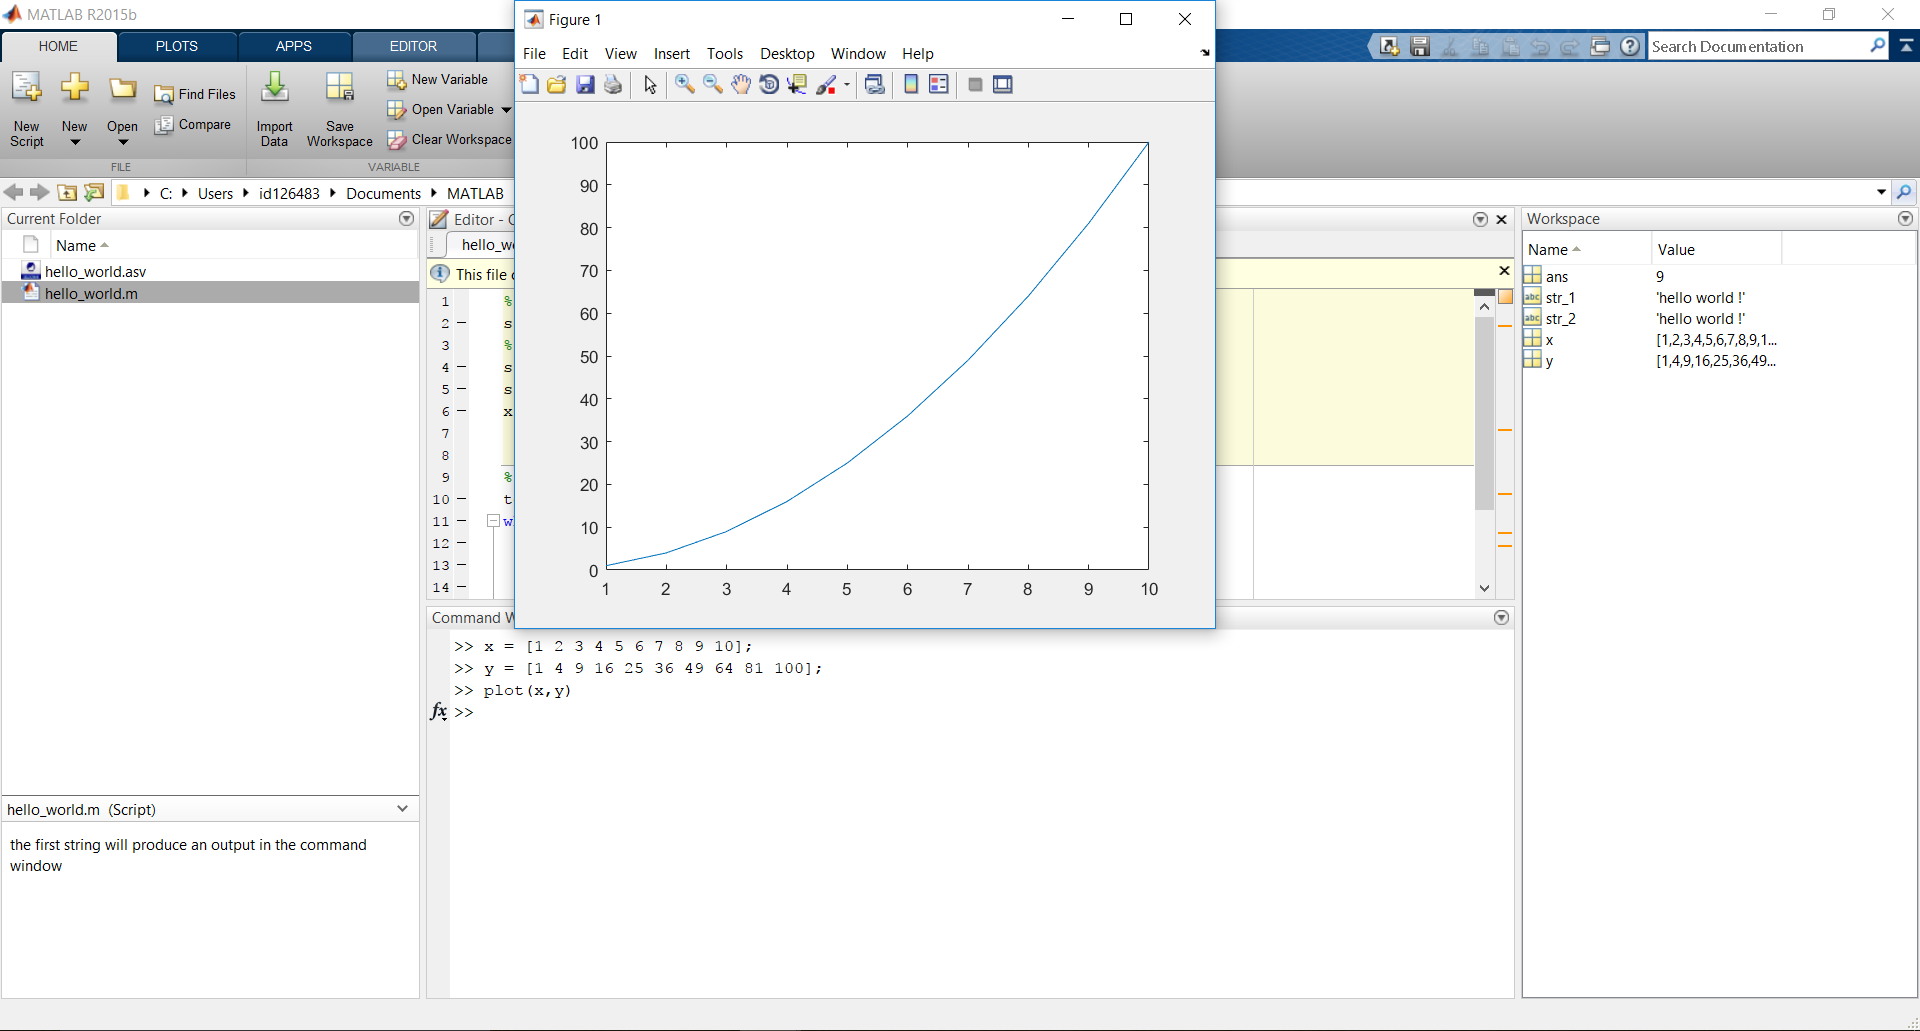
\includegraphics[width=0.95\linewidth]{./fig/plot_1.PNG}
		\caption{
			Plotting some data.
			}
		\label{fig-workspace}
	\end{figure}	
	
	\defbox{Plot}{
		The \mcode{plot} function allows to plot the graph of a function or to plot data.
		
		\begin{itemize}
			\item \mcode{plot(y)} creates a line plot of the data in y.
			\item \mcode{plot(x,y)} creates a line plot of the data in y versus the corresponding values in x.
		\end{itemize}
		\mcode{plot} plots solid lines. To see the data points, one must specify a marker symbol, for example, \mcode{plot(x,y,'o')}.
	}
	\helpbox{plot}
	\tipbox{When only one data is provided, \matlab assumes that the abscisse are the indexes of the elements of the data. 

		What will be plotted is hence the coordinates $(1,y(1)), (2,y(2), \hdots , (n, y(n))$.

		Compare \mcode{plot(x,y)} and \mcode{plot(y)}!

		When trying to understand some results, never hesitate to plot some data \mcode{y} by typing \mcode{plot(y)} in the command prompt. Quick and dirty, but useful.
	}
	\tipbox{
		The command \mcode{figure} can be used for opening a new \emph{empty} figure window.

		\matlab draw any new plot in the last active figure window, erasing the old figure. 
		Creating a new window \emph{before plotting} ensures that the previous plot will not be lost:\\
		\mcode{figure ; plot(x,y)}
	}


%%%%%%%%%%%%%%%%%%%%%%%%%%%%%%%%%%%%%%%%%%%%%%%%
%%%%%%%%%%%%%%%%% SECTION %%%%%%%%%%%%%%%%%%%%%%
%%%%%%%%%%%%%%%%%%%%%%%%%%%%%%%%%%%%%%%%%%%%%%%%
\section{A beautiful plot}
	%%
	% subsection
	%%
	\subsection{What a figure should be}
		A good figure has {\color{red} \large always}:
		\begin{itemize}
			\item labels on the x-axis and y-axis
			\item different colors or patterns for different curves\\ If possible, these differences should persist when printing the figure in black and white.
		\end{itemize}
		If the figure is in a report :
		\begin{itemize}
			\item instead of a title, the figure can be explained in the text under the figure.
			\item instead of a legend, the difference between curves can be explained in the text under the figure.
		\end{itemize}
	\begin{figure}
		\center
		\fbox{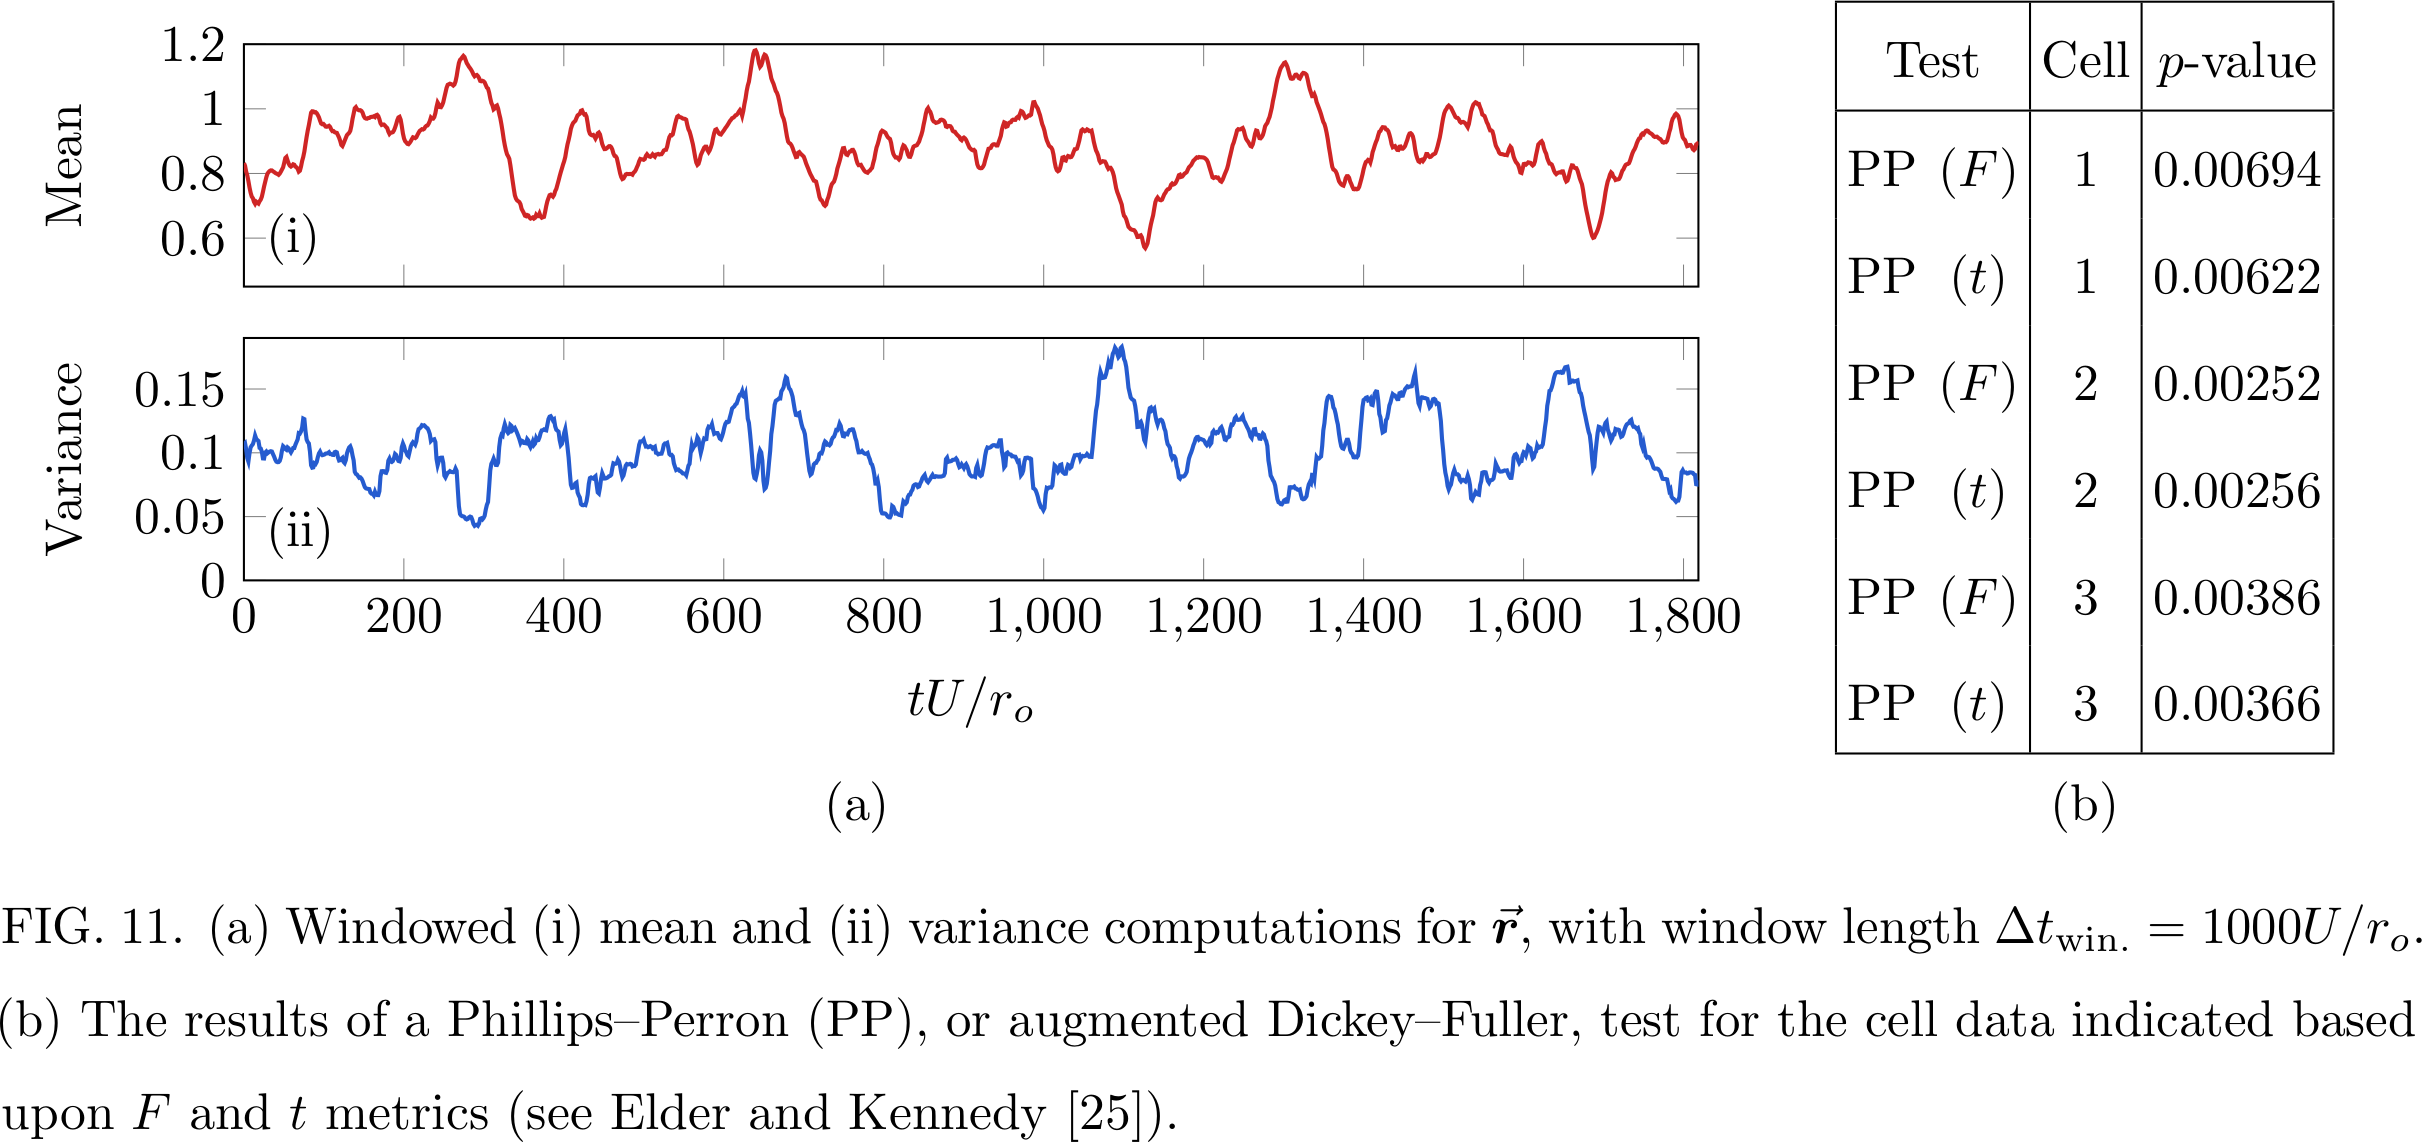
\includegraphics[width=0.95\linewidth]{./fig/beautiful_plot.png}}
		\caption{
			Illustration from a (soon) published paper. Details are provided in the caption, so titles/legends are not necessary. Labels, on the contrary, are always necessary.
			}
		\label{fig-beautiful_plot}
	\end{figure}	
	%%
	% subsection
	%%
	\subsection{axis}
		It is \emph{really important} to always have labels for the axis.
\begin{lstlisting}
>> x = [1 2 3 4 5 6 7 8 9 10];
>> y = [1 4 9 16 25 36 49 64 81 100];
>> plot(x,y)
>> xlabel('data along x')
>> ylabel('data along y')
\end{lstlisting}
		\mcode{xlabel} and \mcode{ylabel} are the \matlab functions that handle the labels.

		The argument for these functions are between quotes "'".
		A label is some text: it means that \matlab will need a string.
\begin{lstlisting}
>> x = 0:pi/10:4.*pi;
>> y = cos(x);
>> plot(x,y)
>> str_xlabel = 'x';
>> xlabel(str_xlabel)
>> str_ylabel = 'cos(x)';
>> ylabel(str_ylabel)
\end{lstlisting}
		\begin{figure}
			\center
			\subfigure[]{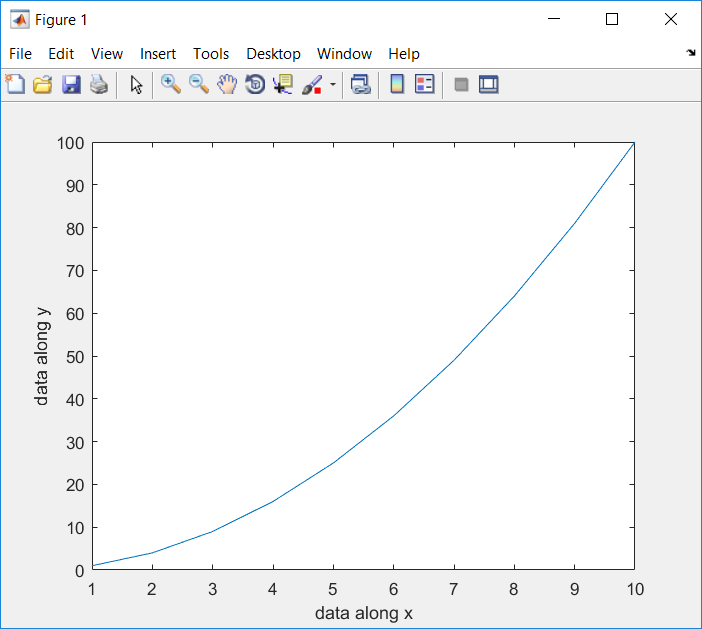
\includegraphics[height=0.43\linewidth]{./fig/plot_label.PNG}\label{subfig-label1}} 
			\subfigure[]{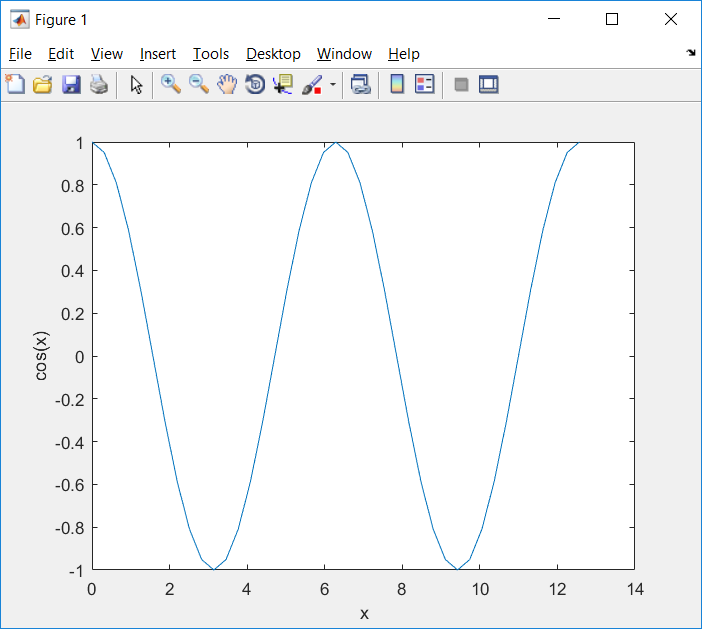
\includegraphics[height=0.43\linewidth]{./fig/cosx.PNG}\label{subfig-label2}}
			\caption{
				Note the labels on these two plots.
				a): plot of the function $f(x) = x^2$ between $1$ and $10$.
				b): plot of $\cos$ between $0$ and $4\pi$.
				}
			\label{fig-labels}
		\end{figure}	
		\subsubsection{Colours and line styles}
			The default plot color in \matlab is blue, and the line default style is plain.
			To change the style, an extra argument has to be sent to \matlab.
			
			For instance, 
			\begin{itemize}
				\item \mcode{plot(x,y,'r')} will change the color of the plot to red.
				\item \mcode{plot(x,y,'--')} will change the line style of the plot to dashed.
			\end{itemize}
			Note that the argument is between quotes.
			Arguments are generally passed as a string
			\begin{table}[h!]
				\caption{A few colours in \matlab.}
				\label{tab-col}
				\center
				\begin{tabular}{|l|c|l|}
					\hline
					colours & code & illustration \\
					\hline
					black & k & \mcode{plot(x,y,'k')} \\
					green & g & \mcode{plot(x,y,'g')} \\
					red & r & \mcode{plot(x,y,'r')} \\
					blue & b & \mcode{plot(x,y,'b')} \\
					yellow & y & \mcode{plot(x,y,'y')} \\
					\hline
					\hline
				\end{tabular}
			\end{table}

			\begin{table}[h!]
				\caption{A few line styles in \matlab.}
				\label{tab-lines}
				\center
				\begin{tabular}{|l|c|l|}
					\hline
					style & code & illustration \\
					\hline
					solid & - & \mcode{plot(x,y,'-')} \\
					dashed & -- & \mcode{plot(x,y,'--')} \\
					dotted & : & \mcode{plot(x,y,':')} \\
					dash-dot & -. & \mcode{plot(x,y,'-.')} \\
					\hline
					\hline
				\end{tabular}
			\end{table}

			\begin{table}[h!]
				\caption{A few marker styles in \matlab.}
				\label{tab-marker}
				\center
				\begin{tabular}{|l|c|l|}
					\hline
					marker & code & illustration \\
					\hline
					plus & + & \mcode{plot(x,y,'+')} \\
					cross & x & \mcode{plot(x,y,'x')} \\
					circle & o & \mcode{plot(x,y,'o')} \\
					triangle up & \^{} & \mcode{plot(x,y,'\^{}')} \\
					triangle down & v & \mcode{plot(x,y,'v')} \\
					triangle left & \textless & \mcode{plot(x,y,'<')} \\
					triangle right & \textgreater & \mcode{plot(x,y,'>')} \\
					\hline
					\hline
				\end{tabular}
			\end{table}
			\tipbox{
				A good way of not messing with the style is to follow this order:
				\begin{enumerate}
					\item open the quotes: \mcode{'}
					\item add the color, e.g. k: \mcode{'k}
					\item add the style of the line, e.g. \mcode{--}: \mcode{'k--}
					\item add the style of the markers, e.g. x: \mcode{'k--x}
					\item end the quotes: \mcode{'k--x'}
				\end{enumerate}
				One will then plot with the options:\\
				\mcode{plot(x,y,'k--x')}
			}

	%%
	% subsection
	%%
	\subsection{Title}
		Adding the title is simple.
		In the same spirit of the labels, just pass the title to the function \mcode{title}.
\begin{lstlisting}
>> x = [1 2 3 4 5 6 7 8 9 10];
>> y = [1 4 9 16 25 36 49 64 81 100];
>> plot(x,y)
>> xlabel('data along x')
>> ylabel('data along y')
>> title ('example of a title')
\end{lstlisting}
		\begin{figure}
			\center
			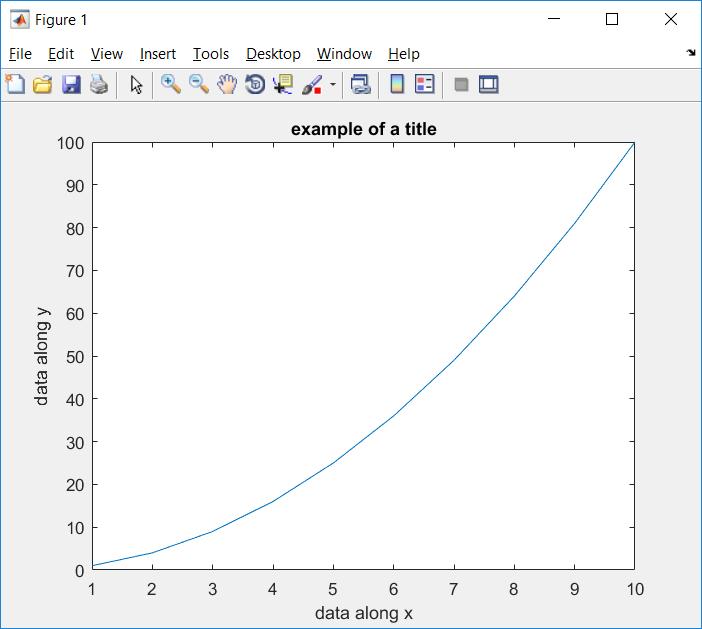
\includegraphics[height=0.43\linewidth]{./fig/plot_title.PNG}
			\caption{
				Note the title.
				}
			\label{fig-title}
		\end{figure}	
%%%%%%%%%%%%%%%%%%%%%%%%%%%%%%%%%%%%%%%%%%%%%%%%
%%%%%%%%%%%%%%%%% SECTION %%%%%%%%%%%%%%%%%%%%%%
%%%%%%%%%%%%%%%%%%%%%%%%%%%%%%%%%%%%%%%%%%%%%%%%
\section{Edit a plot in the window}
	A way to edit the plot properties is to click on the arrow - Edit Plot - on the plot window.

	\begin{figure}[h!]
		\center
		\begin{tikzpicture}
			\node at (0,0) { 
				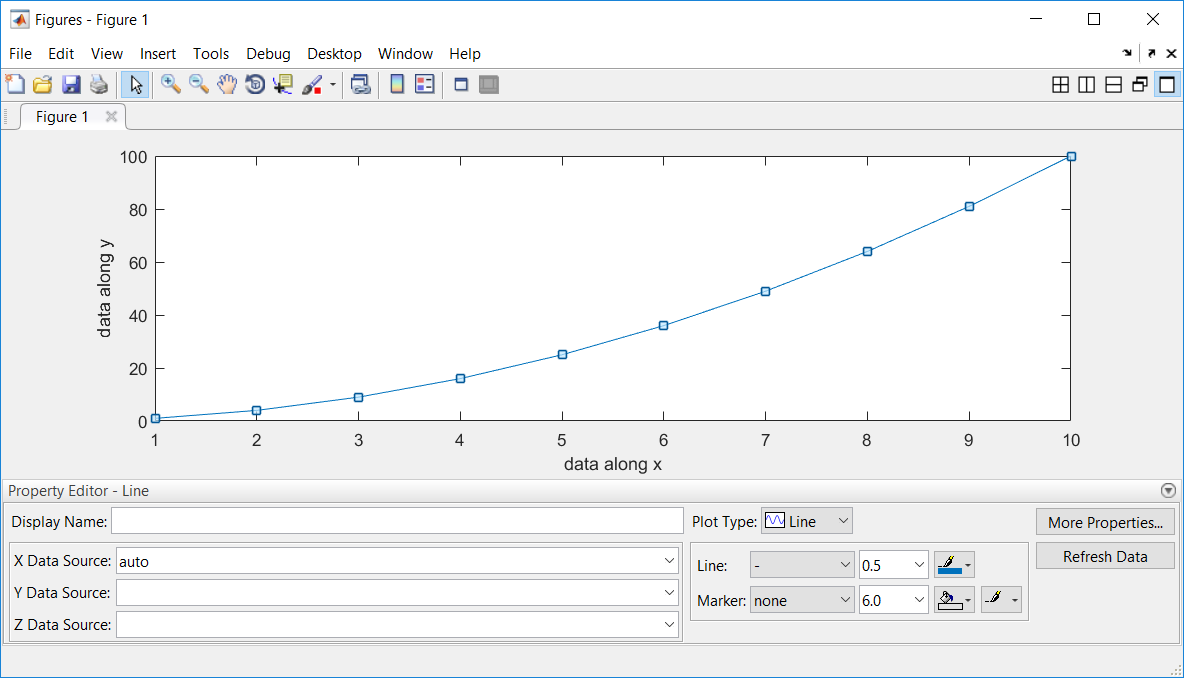
\includegraphics[width=0.9\linewidth]{./fig/plot_edit.PNG}
			};
			\draw[very thick,red,->] (-3.,.75) -- ++(-2,2) node[midway, below,rotate=-45]{click here};
			\draw[very thick,red,->] (3.2,.45) -- ++(-1.5,0) node[midway, below]{then on the graph};
			
		\end{tikzpicture}
		\caption{
			Editing a plot from the window is relatively simple, though fastidious.
			First click on the "arrow" to start the edit mode. 
			Then, clicking on one of the plot objects, for instance, the curve, will allow to start editing it. 
			Note the \mcode{Line} and \mcode{Marker} properties.
			}
		\label{fig-edit}
		\end{figure}	
	Then, double clicking on the curve will open an extra window where one can play with the properties.

	In particular there is two interesting properties:
	\begin{enumerate}
		\item \mcode{Line}, where the style of line can be edited (plain, dashed, etc.), the width of the line, and its color
		\item \mcode{Marker}, where the type of markers can be edited (indication where each data is plotted, for instance with circles), the size of the markers, the color of the inside of the marker as well as the color of their edges
	\end{enumerate}

%%%%%%%%%%%%%%%%%%%%%%%%%%%%%%%%%%%%%%%%%%%%%%%%
%%%%%%%%%%%%%%%%% SECTION %%%%%%%%%%%%%%%%%%%%%%
%%%%%%%%%%%%%%%%%%%%%%%%%%%%%%%%%%%%%%%%%%%%%%%%
\section{Multiple plots}
	%%
	% subsection
	%%
	\subsection{Multiple plot in one figure}
		\subsubsection{In one call}
			One call to the function \mcode{plot} is enough to plot multiple graphs on the same figure.
			For that, couple of arguments need to be provided to the \mcode{plot} function.
\begin{lstlisting}
>> x = 0:0.1:4.*pi
>> y_1 = cos(x); y_2 = cos(x+0.8); y_3 = cos(x+1.6);
>> plot(x,y_1,x,y_2,x,y_3)
>> xlabel('x')
>> ylabel('f(x)')
>> title ('several cos')
\end{lstlisting}
			To add some control on the plot, the style can be provided just after the data:
\begin{lstlisting}
>> plot(x,y_1,'-',x,y_2,':',x,y_3,'--')
>> legend('cos(x)','cos(x+0.8)','cos(x+1.6)')
\end{lstlisting}

		\begin{figure}
			\center
			\subfigure[]{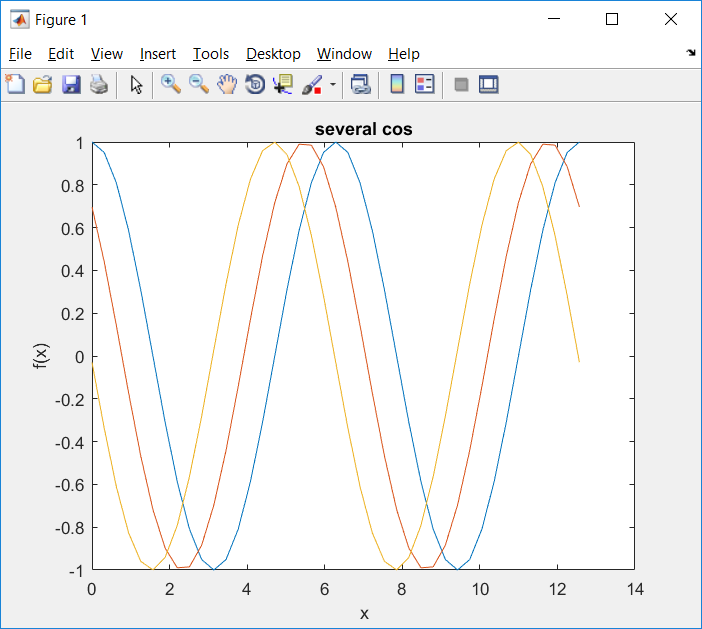
\includegraphics[height=0.43\linewidth]{./fig/multi_plot1.PNG}\label{subfig-multi1}} 
			\subfigure[]{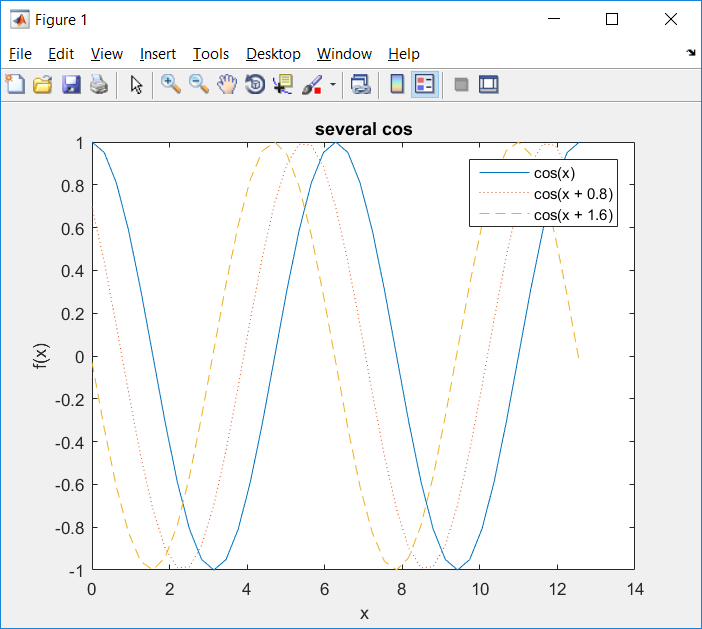
\includegraphics[height=0.43\linewidth]{./fig/multi_plot_style.PNG}\label{subfig-multi2}}
			\caption{
				Several graph on the same figure.
				a): no style is provided. 
				b): "stylish" curves.
			}
			\label{fig-multi}
		\end{figure}	
		\subsubsection{In multiple call}
			When calling \mcode{plot}, the active figure gets erased before \matlab draw the new plot.
			
			But calling \mcode{hold on} (and later on \mcode{hold off}) \matlab knows that it should not erase the figure.
\begin{lstlisting}
>> x = 0:0.1:2.*pi
>> y_1 = cos(x); y_2 = cos(x+0.2); y_3 = cos(x+0.4);
>> plot(x,y_1)
>> hold on
>> plot(x,y_2)
>> plot(x,y_3)
>> hold off
\end{lstlisting}
			\mcode{hold off} tell \matlab that the figure is no longer protected.

	%%
	% subsection
	%%
	\subsection{figure and multiple plots}
			\todoimage{plot}

		\todo{this section}

	%%
	% subsection
	%%
	\subsection{legends}
		Adding the legend is simple.
		In the same spirit of the title, just pass the legends, one after the other, to the function \mcode{legend}:
\begin{lstlisting}
>> plot(x,y_1,'-',x,y_2,':',x,y_3,'--')
>> legend('cos(x)','cos(x+0.2)','cos(x+0.4)')
\end{lstlisting}

		\begin{figure}
			\center
			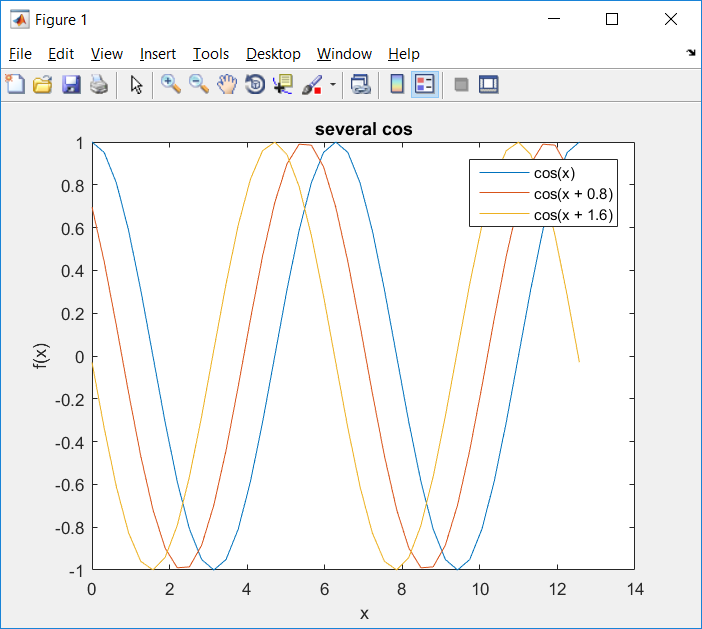
\includegraphics[height=0.43\linewidth]{./fig/multi_plot_legend.PNG} 
			\caption{
				Same figure as before, with legends.
			}
			\label{fig-legend}
		\end{figure}	






\chapter{Programming}
\label{chap-code}

%%%%%%%%%%%%%%%%%%%%%%%%%%%%%%%%%%%%%%%%%%%%%%%%
%%%%%%%%%%%%%%%%% SECTION %%%%%%%%%%%%%%%%%%%%%%
%%%%%%%%%%%%%%%%%%%%%%%%%%%%%%%%%%%%%%%%%%%%%%%%
\section{Script}\label{sec-script}
	Scripts are the simplest kind of program file because they have no input or output arguments. 

	They are useful for automating series of \matlab commands, such as computations that have to be performed repeatedly from the command line.


	When execution of the script completes, the variables remain in the \matlab workspace. 


	\defbox{Script}{A script is basically a text file, with the ".m" extension, for instance, \mcode{my\_script.m}.
	
		This file contains series of instructions that \matlab can and/or will execute.

		A script does not take inputs (they hence have to be provided). It does not provide outputs, though the variables will be stored in the workspace.
	}
	\todoimage{tikz illustration of a script?}

	%%
	% subsection
	%%
	\subsection{Create a script}
		One can create a new script in the many ways.
		
		\subsubsection{Creating a script with the prompt}
			The \mcode{edit} command allows either to create a script, or to edit an existing script.
			To create a blank script, named "untitled.m", type:
\begin{lstlisting}
>> edit
\end{lstlisting}
			\matlab will then create and open the script.
			The script is created in the current folder that \matlab is using. 
			To change the folder, the "current directory" windows on the left should be used.
		
			To create a script named "my\_scipt.m", type:
\begin{lstlisting}
>> edit my_script
\end{lstlisting}
			Note that specifying the extension is unecessary.
			Also, when the script "my\_script.m" exists already, typing \mcode{edit my\_script} will open the preexisting script.		
		\subsubsection{Through \matlab interface}
			Another way is through the IDE.
			Click on the "EDITOR" tab, then on "+ New", and select script.
			One can then save it with the desired name.

		\subsubsection{Create a text file}
			Just create a text file (file with the ".txt" extension) in windows, and change the extension to ".m".

		Et voilà.

	%%
	% subsection
	%%
	\subsection{Save a script}
		Saving a script and running the code can be done using either of these methods:
		\begin{itemize}
			\item Typing the script name on the command line and pressing Enter. 
			\item Clicking the Run button on the Editor tab.
			\item Clicking on the save icon.
		\end{itemize}

	%%
	% subsection
	%%
	\subsection{Comments}
		On of the most important thing is to always try write as much comments as possible in a code.

		\defbox{Comment}{
			A comment is a part of the file that will \emph{not} be executed by \matlab.
			It allows to give explanations on the script. 
			For later reading, or if someone else is reading the code, it will give invaluable information on what the code is actually doing.

			Any line starting with the percentage symbol "\%" will be ignored.
			Any part between "\%\{"  and "\%\}" will be ignored as well.
			}
			\tipbox{
				A good piece of code needs:
				\begin{itemize}
					\item well-named variables
					\item indentation
					\item comments
				\end{itemize}
			}

	\subsection{execute the script}
		There is several way for running a script, from the editor, from the prompt and thanks to convenient shortcuts.
		\subsubsection{From the editor}
			\paragraph{Run button}
				The easiest is to be in the editor and to click on the triangle button "\textgreater".
				\todoimage{run button}
				\begin{figure}
					\center
						\begin{tikzpicture}
							\node at (0,0) {
								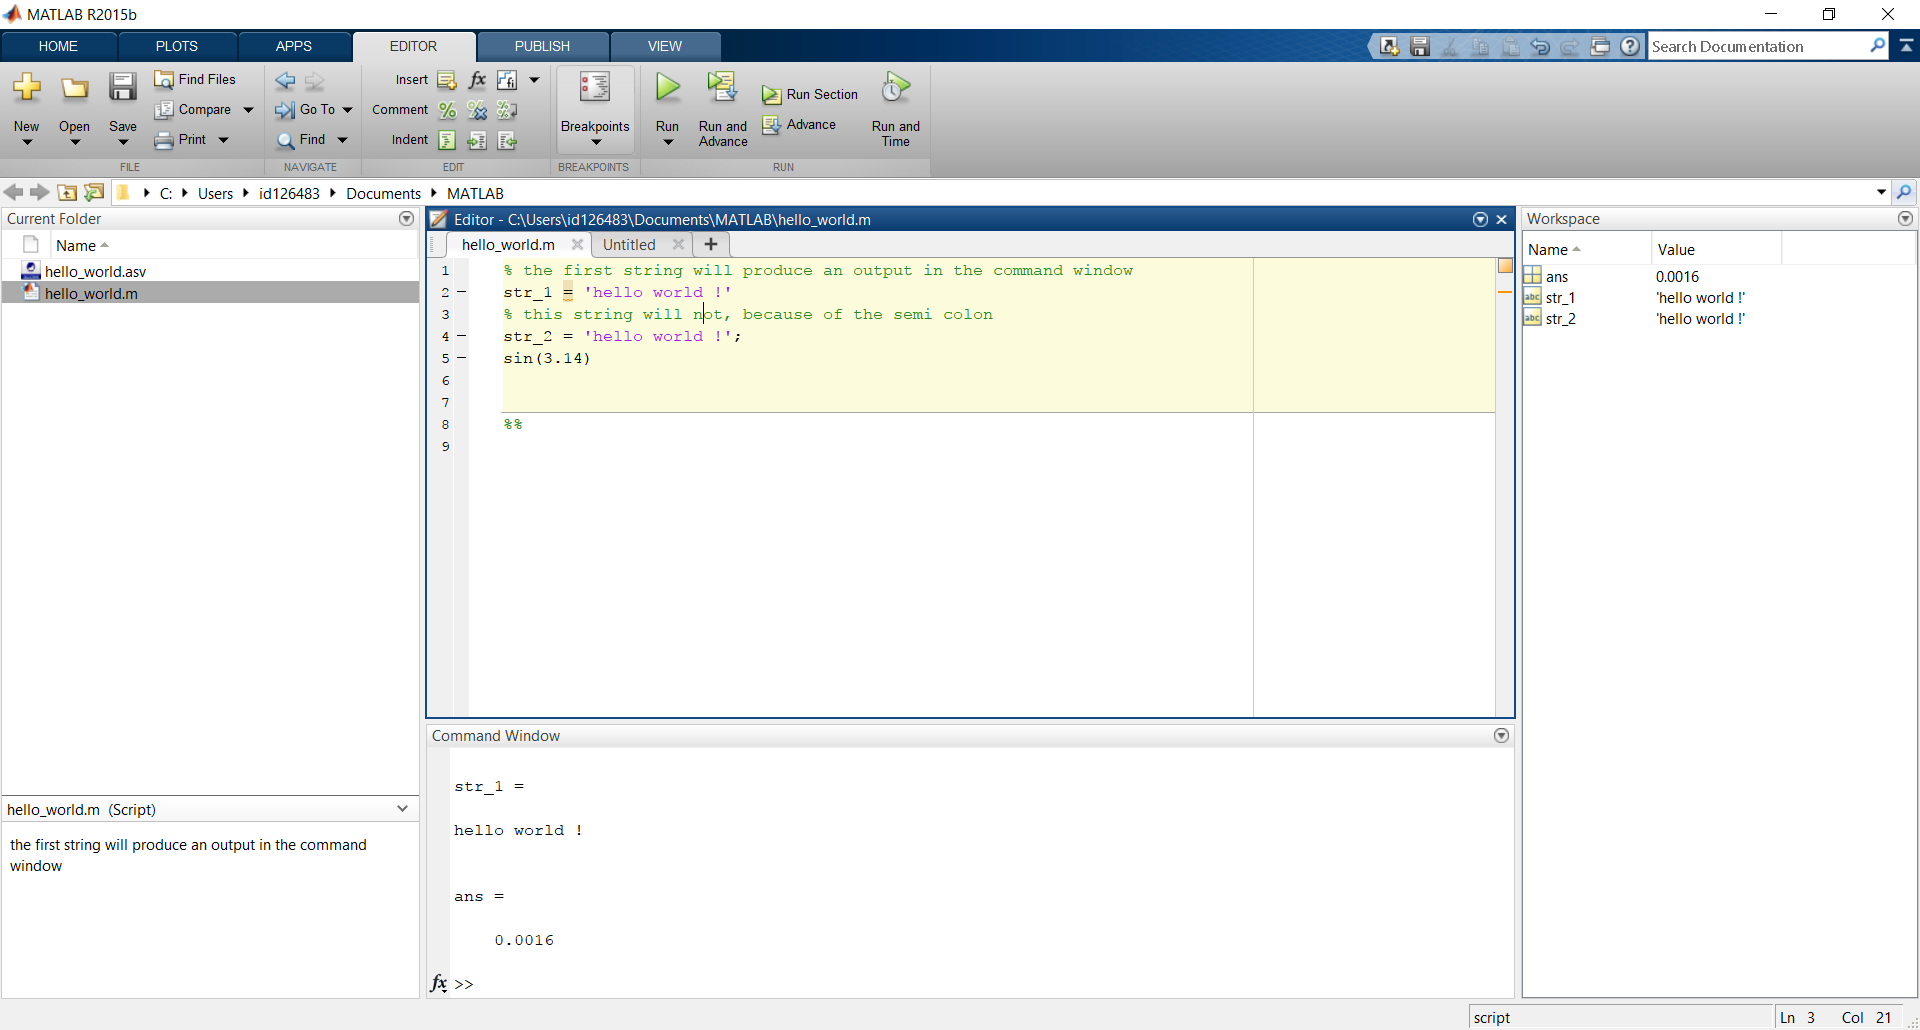
\includegraphics[width=0.95\linewidth]{./fig/editor_run.PNG}
							};
							\draw[very thick, red, ->] (-4.25,1) -- ++(2,2) node[above, midway, rotate=45,fill=white]{Run button};
						\end{tikzpicture}
			\caption{
				the run button in the editor.
			}
			\label{fig-run}
		\end{figure}	

				It will run the whole script (and will save it).
		
			\paragraph{Shortcut}
				There is two extremely handy shortcuts, from the editor:
				\begin{enumerate}
					\item \mcode{F5} will run the whole script
					\item \mcode{ctrl+enter} will run the active cell
				\end{enumerate}
				The last one is really convenient as well.
				The active cell is highlighted in light yellow.

			\subsubsection{From the prompt}
			Another easy way is to type the name of the script:
\begin{lstlisting}
>> my_script
\end{lstlisting}
			Alternatively, the function \mcode{run} can be used:
\begin{lstlisting}
>> run my_script
\end{lstlisting}

	\subsection{reading the script}
		\matlab has a set of colors for helping the reader to understand the code:
		\begin{itemize}
			\item green: comments
			\item blue: functions (to be verified)
			\item yellow background: section with focus
		\end{itemize}


%%%%%%%%%%%%%%%%%%%%%%%%%%%%%%%%%%%%%%%%%%%%%%%%
%%%%%%%%%%%%%%%%% SECTION %%%%%%%%%%%%%%%%%%%%%%
%%%%%%%%%%%%%%%%%%%%%%%%%%%%%%%%%%%%%%%%%%%%%%%%
\section{Loops}
	Loop control statements will repeatedly execute a block of code.
	It is really convenient, as sometimes, one want to do \emph{almost} the same thing many times.
	For instance, evaluating a series, such as the Fibonacci sequence, one needs to evaluate repeatedly the same expression $un = u_{n-1} + u_{n-2}$.




	There are two types of loops:
	\begin{itemize}
		\item \mcode{for} statements loop a specific number of times, and keep track of each iteration with an incrementing index variable.
		\item \mcode{while} statements loop as long as a condition remains true.
	\end{itemize}
	\defbox{Loop}{
		A loop will repeat instructions a certain number of times.

		It is really useful when something can be done almost exactly similarly from on time to the other.
		For instance, if one want to compute the distance that Julie (see Sec.~\ref{problem-julie}) can drive if the tank is 20 liters, 25 liters ? or maybe if it is 55 liters ?

		One can loop on the variable \mcode{tank\_capacity} and not have to rewrite the code several times or to execute it several times.
	}
	\todoimage{tikz illustration of a loop}
	
	%%
	% subsection
	%%
	\subsection{Loops based on For}
		\mcode{for} loops are based on a finite number of iterations.

		Executing this script:
\begin{lstlisting}
for i=1:5,
  i
end
\end{lstlisting}
		will lead in print i at every step of the loop. 
		\mcode{i} will hence be 1 then 2 etc. up to 5.
		\defbox{for}{
			A \mcode{for} statement will execute a block of code repeatedly.


			What is needed for making a \mcode{for} loop:
			\begin{itemize}
				\item a list \mcode{my\_array}
				\item a variable \mcode{var\_i}
				\item some code \mcode{do stuff}
			\end{itemize}
			
			The \mcode{for} loop is written as:
			\begin{enumerate}
				\item \mcode{for var\_i=my\_array,} 
				\item \mcode{do stuff}
				\item \mcode{end}
			\end{enumerate}
			First, \mcode{var\_i} will, one after the other, be assigned to every value that exists in \mcode{my\_array}.
		If \mcode{my\_array=[1,2,3]}, then \mcode{var\_i} will be 1, then 2, then 3.\\

		Once \mcode{var\_i} has been assignated to a new value, \matlab will execute the code \mcode{do stuff}.
		If \mcode{do stuff} is $i^2$, then \matlab will print $1$, then $4$, and finally $9$.
\\

		\mcode{end} says to \matlab that the part \mcode{do stuff} is finished and that he can loop.\\

		\mcode{do stuff} can be very complex instructions, and \mcode{my\_array} can be a very long list, for instance \mcode{1:10000}.
			}
		A useful example is construction of vectors.
		Let's for instance construct the Fibonacci sequence up to 100:
\begin{lstlisting}
fibo = ones(100);
for i=3:100,
  fibo(i) = fibo(i-2) + fibo(i-1);
end
\end{lstlisting}
		It is possible to nest loops, i.e., to have a loop in a loop. 
		Let's construct a Vandermonde matrix.
\begin{lstlisting}
v = 1:4;
M = ones(4,4);
for i=1:4,
  for j=1:4,
    M(i,j) = v(i)^j;
  end
end
\end{lstlisting}
		\tipbox{
			Indent the loops for readability!

			For each loops, indent by using tab or a few spaces.

			Without indentation, it is really hard to see when loops start and end.
		}


	\subsection{Loop based on while}
		
	\subsection{Controls on loops}
		Exiting a loop can be done programmatically by using a break statement, or skip to the next iteration of a loop using a \mcode{continue} statement.  Details will be given in Sec.~\ref{sec-if}



%%%%%%%%%%%%%%%%%%%%%%%%%%%%%%%%%%%%%%%%%%%%%%%%
%%%%%%%%%%%%%%%%% SECTION %%%%%%%%%%%%%%%%%%%%%%
%%%%%%%%%%%%%%%%%%%%%%%%%%%%%%%%%%%%%%%%%%%%%%%%
\section{Conditions}\label{sec-if}
	\subsection{Is $x>0.5$?}
	\tipbox{
		Checking is a quantity is equal to an other is \emph{very} important.
		
		For instance, it is pivotal in \mcode{if/else} statements. 
		The condition has to be checked. Is it true or false ?

		But \matlab can not understand \emph{condition} = true. 
		That would assign true to the condition, which is \emph{very} different from checking if the condition is true.

		Consequently, \matlab uses a special operator for checking if two quantities are equal: the "==" operator.
	}
	\todo{work here}	

	\subsection{\mcode{if/else} statement}
	More than often, computations depend on the situation. 
	Think of a piece-wise function, define on $[0,1]$:
	$$f(x) = \left\{\
		\begin{array}{c}
			-1 \text{if } x<0.5\\
			 1 \text{if } x>0.5
		\end{array}
		\right.
	$$
	Evaluating $f$ hence depends if the argument $x$ is larger or lesser than $0.5$.
	The keyword is \mcode{if}.

	\defbox{if/else}{
		The \mcode{if/else} statement executes a block of code if a specified condition is true. If the condition is false, another block of code can be executed.

		What is needed for making a \mcode{for} loop:
		\begin{itemize}
			\item specified \emph{condition} to be verified
			\item some code \mcode{do stuff} if the \emph{condition} is true
			\item some other code \mcode{do other stuff} if the \emph{condition} is false
		\end{itemize}
	
		The \mcode{if/else} statement is written as:
		\begin{enumerate}
			\item \mcode{if} \emph{condition} \mcode{== True,}
			\item \mcode{do stuff}
			\item \mcode{else,}
			\item \mcode{do other stuff}
			\item \mcode{end}				
		\end{enumerate}

		If there is no block \mcode{do other stuff} then the statement is slightly simpler:
		\begin{enumerate}
			\item \mcode{if} \emph{condition} \mcode{== True,}
			\item \mcode{do stuff}
			\item \mcode{end}				
		\end{enumerate}
	
		First, \matlab will check if the condition is true. 
		For instance, the condition can be $x$ larger than $0.5$.
		The condition then writes \mcode{x>0.5}.
		The first part, corresponding to the evaluation, of the \mcode{if/else}  statement is then: \mcode{if (x>0.5) == true,}.
		Then, \mcode{do stuff} is executed if the \emph{condition} is true. 
		For instance, the variable \mcode{fx} can be assigned to 1, with the piece of code \mcode{fx = 1;}.
		Then, if specified and in the eventuality than the \emph{condition} is false, the alternative code can be executed, say that \mcode{do other stuff} is to assign -1 to the variable fx: \mcode{fx = -1}.
		Finally, the \emph{end} statement will tell \matlab that the \mcode{if/else} block is finished.
	}


	Understanding if requires to understand 
\begin{lstlisting}
x = 0.6
if (x>0.5) == true,
	fx = 1;
else,
	fx = -1;
end
\end{lstlisting}

	%\subsection{\mcode{switch} statement}

\bibliographystyle{ieeetr}
\bibliography{biblio}

\end{document}

%%
%% End of file `elsarticle-template-3a-num.tex'.
